% !Mode:: "TeX:UTF-8" 

\BiChapter{研究可编程设备加速网络硬件交换层方法}{Switch} %15页


\BiSection{本章引论}{aa}


\BiSection{问题背景}{aa}

可编程网络硬件可以运行传统部署在服务器内的功能,从而将网络性能提高数个量级。由于软件定义网络概念的提出,网络灵活性增强,运营商更倾向于自主管理网络内设备的所有行为。具有灵活性的管理方式可以大大增加网络的运行效率,为特定的功能定制专用的网络场景。  现有的面向网络通信的可编程数据平面一般有x86平台,开放接口配置的ASIC转发芯片,以及上一章本文提到的FPGA平台。他们在处理灵活性,转发性能等方面均有长足进步,但正如本文第二章中介绍,在面对转发容量进一步增强,灵活性需求进一步开放的网络应用时依然面临新的挑战:

1)软件具有高度灵活性,但处理性能低下。

数据包交换对于CPU架构平台来说是一种很低效的机械劳动。在软件层面,数据包转发算法已经被优化的极为高效,但面对无穷无尽的任务量,依靠CPU指令集的处理架构存在访存效率低、无法批处理等问题。CPU无法发挥自己实现灵活程序跳转、分支的优势,因此目前高性能软件网络处理性能也只能达到10Gbps(单核心)。对于现代服务器面向200G接口,汇聚层交换转发动辄5、6Tbps的性能需求是远远无法满足的。

2)基于FPGA可编程硬件平台。

FPGA是一种逻辑可编程芯片,可提供软件一般的灵活性也具有硬件的性能。目前,主要的云计算厂商阿里巴巴、亚马逊、微软都在数据通路内部署了FPGA加速引擎以同时满足性能和灵活性的需求,例如提升网络加解密性能,定制传输层协议等。然而由于FPGA电路编码转换采用“查找表+内部互联网络”的原理,为保证时间同步性,使得FPGA综合对外的处理主频只能达到200MHz,这样即使FPGA内流水线每个周期都能处理一个数据包,总吞吐性能也无法超过100Gbps\citeup{wang2017p4fpga,netfpga2014}。虽强于软件,但远差于网络的核心层性能需求。

3)协议无关概念的交换芯片。

与协议无关交换架构(Protocol-Independent Switch Architecture,PISA)相对应的是P4(Programming Protocol-Independent Packet Processor)。P4是一种专用的编程语言,其目标是为任意包协议提供一种基于ASIC硬件(PISA)的现场可重配置能力。根据本文在第二章的介绍,PISA有能力实现自定义包头解析,自定义流表的组成结构,并且最重要的它拥有最强大的处理能力(12.8Tbps,显然是唯一可以胜任核心转发设备的架构)。虽然这大大解决OpenFlow编程能力不足以及其设计本身所带来的的可扩展性差的难题,但它不具备真正意义上其所追求的“图灵完备”可编程。例如:(1)数据通路内的处理动作只能被数据包触发,而无法响应其他行为。针对一些QoS场景系统更希望根据队列深度做出一些响应,比如拥塞控制场景下的控制算法NDP\citeup{handley2017re};(2)PISA缺乏计算、控制属性的指令集,例如乘除法、灵活分支判断等;(3)PISA为无状态转发的可编程流水线设计,则对状态协议处理以及有状态计算造成了困难(防火墙等)。

PISA转为通用型的无状态转发同时提高了性能与灵活性,本文将对PISA架构芯片的目标处理内容做进一步扩展。本文的目标是设计一种适用于网络交换层的交换机架构,这种架构可从计算平面高灵活性的工作任务分离和卸载到网络中,包含但不限于有状态转发、复杂计算以及自定义触发方式。



\BiSection{系统架构介绍}{aa} 

P4是目前广泛使用的可定义数据平面内的数据包解析和查表过程的语言。P4将流水线外的功能需求通过P4\_extern模块来让用户自行定义。然而P4\_extern的编程范围只在PISA提供的执行器序列之内,例如校验算法,位移,插入数据等。目前的PISA芯片架构对于“PISA\_extern”的功能需求没有支撑能力。一种显而易见的解决方案是当需要一种新的“PISA\_extern”时,重新设计一种支撑新特性执行器的ASIC硬件。但这与PISA高灵活性的设计初衷相矛盾,从经济实用性角度分析也是不合理的。

本文提出一种硬件异构型的交换机架构,可以支持任意P4\_extern所定义的功能。本文将这种结构命名为“自适应交换”,首先本文需要解决如何设计硬件结构使得灵活性和性能可以充分展现,其次本文需要解决如何开发编程语言以映射到自适应交换的数据平面。最终为了展示自适应交换的高扩展性,本文将上小节内提出的PISA难以应用的场景均在自适应交换平台中实现。

\BiSubsection{架构设计}{aa}

\begin{figure}[!ht]
	\centering 
	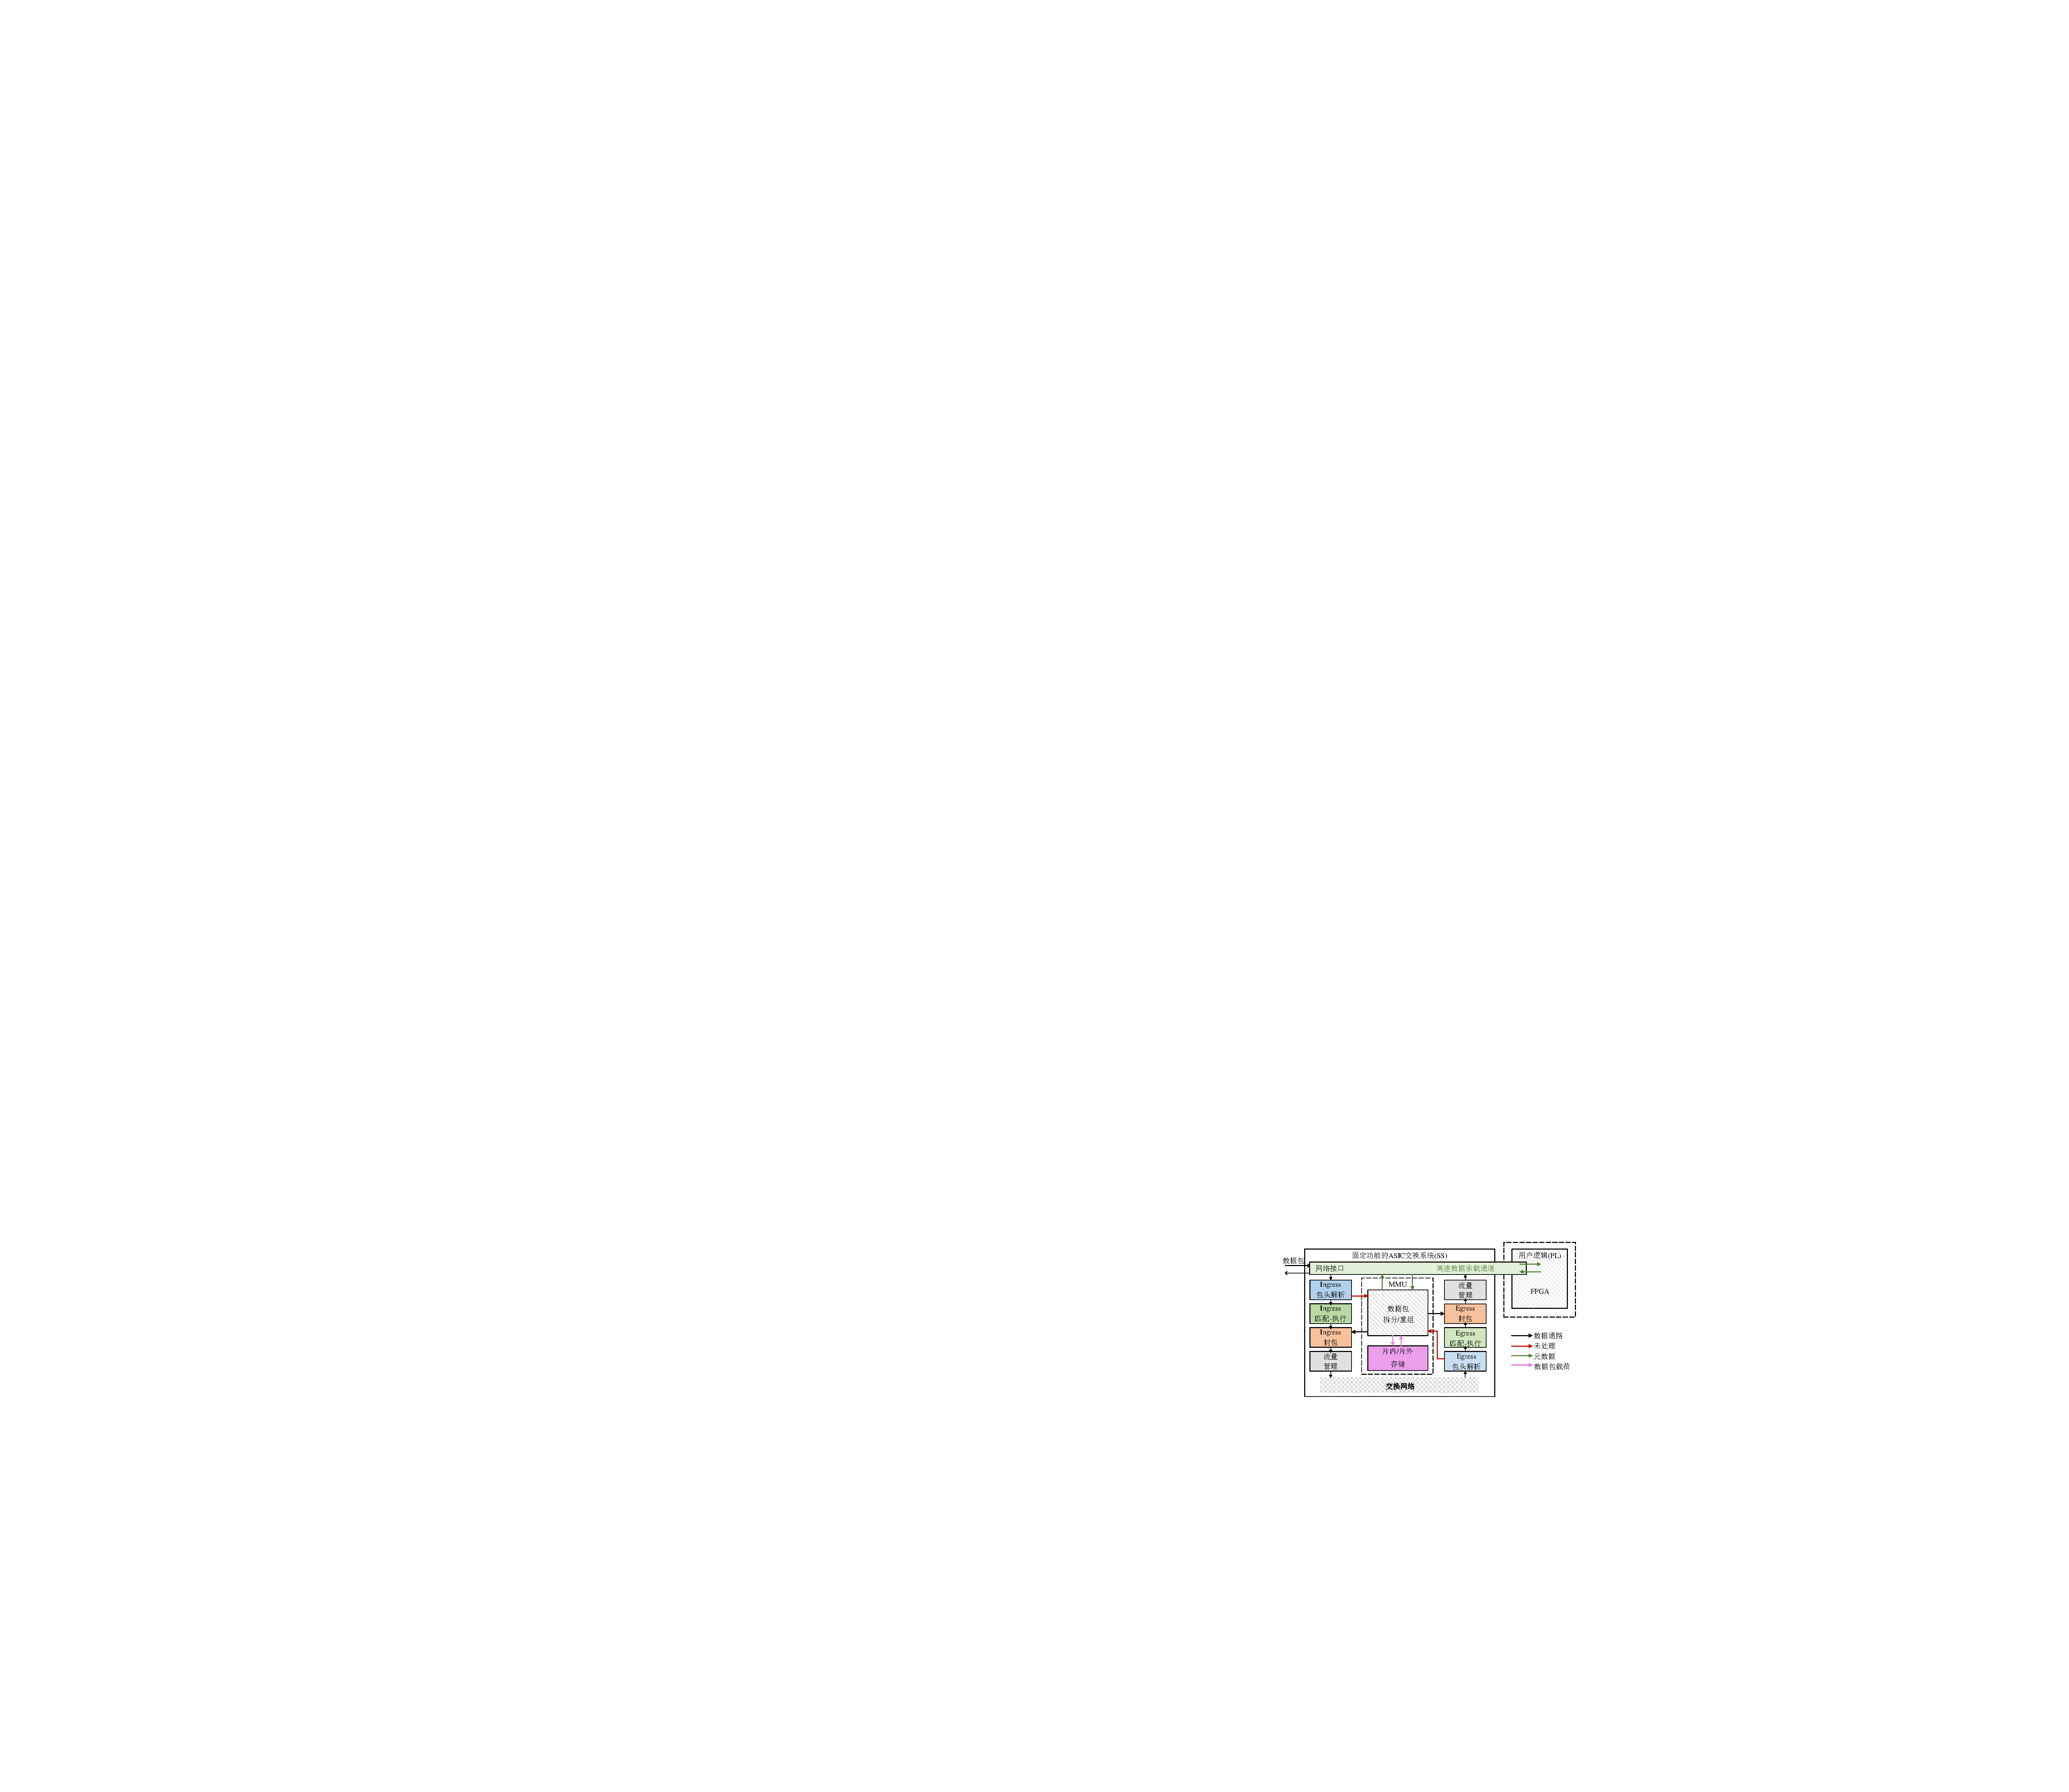
\includegraphics[scale=1]{asarch.pdf}
	\caption{自适应交换结构框图} \label{fig:asarch}
\end{figure}

自适应交换的硬件架构框图。自适应交换包括两部分,1)固定功能的ASIC交换系统(Switching System, SS);2)用户定义可编程逻辑块(Programmable Logic, PL)。SS基于标准的交换芯片(switching ASCI)处理功能,PL利用FPGA类的可编程硬件支持用户自定义逻辑。一个标准的交换芯片功能包含了数据包头的解析,基本的ACL功能和各个字段的匹配以及执行转发/丢包等动作。额外还会包括流量管理、队列调度等QoS功能。架构中SS与PL两部分可由双芯片拼接的方式实现,SS部分利用一个标准传统的交换芯片(既可以支持P4编程,也可以不支持P4编程)构成。PL端使用FPGA芯片或由FPGA构成的多用途片上系统(MPSoC/ACAP)芯片。在双芯片拼接方案中,两个独立的芯片系统须通过高速互联总线相连接,例如PCIe接口,以太网接口或者类似的收发器。相应地自适应交换系统也可以由单独一颗芯片构建而成,PL与SS部分通过片上高速总线相接,例如,AXI协议总线。

如图\ref{fig:asarch}左半部分所示,交换网络是SS的核心组成部分。交换网络支持网络入端接口与出端接口多对多的数据包互联传送,一般由交叉开关(cross-bar)构成。数据包经由物理网络接口进入SS系统,在交换网络两边,数据包会经过入端(Ingress)处理流水线,以及出端(Egress)处理流水线。在两条流水线的组成分别有包头解析(抽取必要的包头域数据),流表(对包头域数据进行匹配和执行相应的动作集),封包(重组/修改数据包结构),以及流量管理(包缓存/调度/限速等)。

数据包进入自适应系统时,首先经由SS端的处理,通常情况下大部分数据包可以完整地被SS处理,并返回外部网络。只有在SS内的功能无法满足需求的那部分数据包会再次送入PL端做协同处理。对于送往PL端处理的数据包,在SS端在片上存储中(或使用片外存储)也保留有一份完整是数据包备份,SS只将数据包的元祖数据信息送给PL。元祖数据中包括了PL完成处理所需要的定制化的包头信息或者其他描述信息。PL处理完成元祖数据后,会更新重写元祖信息中的包头以及描述字段,再返回给SS。最后SS将备份的原始数据包与更新的元祖数据重新整合成一个完整的数据包后再次对其执行转发操作,或简单丢包。

本文将在传统的交换芯片中增加一个包存储管理机制(Memory Management Unit, MMU),图\ref{fig:asarch}中左边虚线内部所示。当数据包元祖信息送往PL处理时,这个数据包在SS端的完整备份由MMU管理。MMU应包含三个主要功能:(1)动态申请/释放数据包的存储块位置及其大小;(2)驱动数据包向内存中读写时序;(3)读出备份数据包后与从PL返回的新元数据对接重组。

上述自适应交换流程与原理是建立在本文对以下两方面的分析结果和假设之上。首先,在PL中处理的信息通常只依赖于包头,或者数据包包首部分的字段。在设计中被交换到PL的元数据可以被灵活地定义,并且保证只占用SS与PL之间一定量的通信带宽成本。在某些极端的例子中,如果处理过程需要数据包所有的数据时,元祖数据也将会包含一个完整的数据包内容。第二,不是所有的数据包处理都需求调用PL端的功能。否则,如果有一种功能是普遍适用的,则一定会集成在现行的通用交换芯片内。或者这种功能需求可以直接拆分出来一部分由SS端完成处理。

自适应交换的高性能来自于对网络通用数据包包长的分析。本文考虑到,目前网络内平均包长度为600字节左右,假设元祖数据包含整个包头部分(64字节之内),则SS与PL之间的通信成本只占需求流量的10\%。即,利用单插槽的PCIe4.0接口(256Gbps)作为高速互联,自适应交换系统可以将目前最高速度(12.8Tbps)交换芯片中20\%的数据(>2Tbps)卸载到用户硬件可编程逻辑中进行处理。这远远超过了($\times$10倍)单纯由FPGA组成的可编程数据平面的处理性能,也是本文研究的最主要的动机。

\BiSubsection{开发流程}{aa}

对于基于FPGA的PL端,基本的开发设计流程包括如下几部分:

\begin{itemize}
	\item 定义数据包处理需求以及所需要的数据流模型。
	\item 编写处理规则对应的函数或流程代码。程序代码可包括高级语言如P4/P4\_extern、P4\_FPGA,或者底层的硬件描述语言如verilog HDL。此外包括数据平面高层次生成系统,如SDNet\citeup{sdnet},也可以用于加速PL端的开发工作。
	\item PL端的机器码编译器。不同PL目标器件下的编程,往往有不同的编译步骤。对于基于FPGA的编译器,本文使用FPGA芯片厂商提供的编译环境。但本文最主要的贡献是解决如何将数据包流处理模型在异构形态下重新组织,并且完成高性能的异构形态下包处理逻辑无语义偏差的拆分和翻译。
\end{itemize}

\begin{figure}[!ht]
	\centering 
	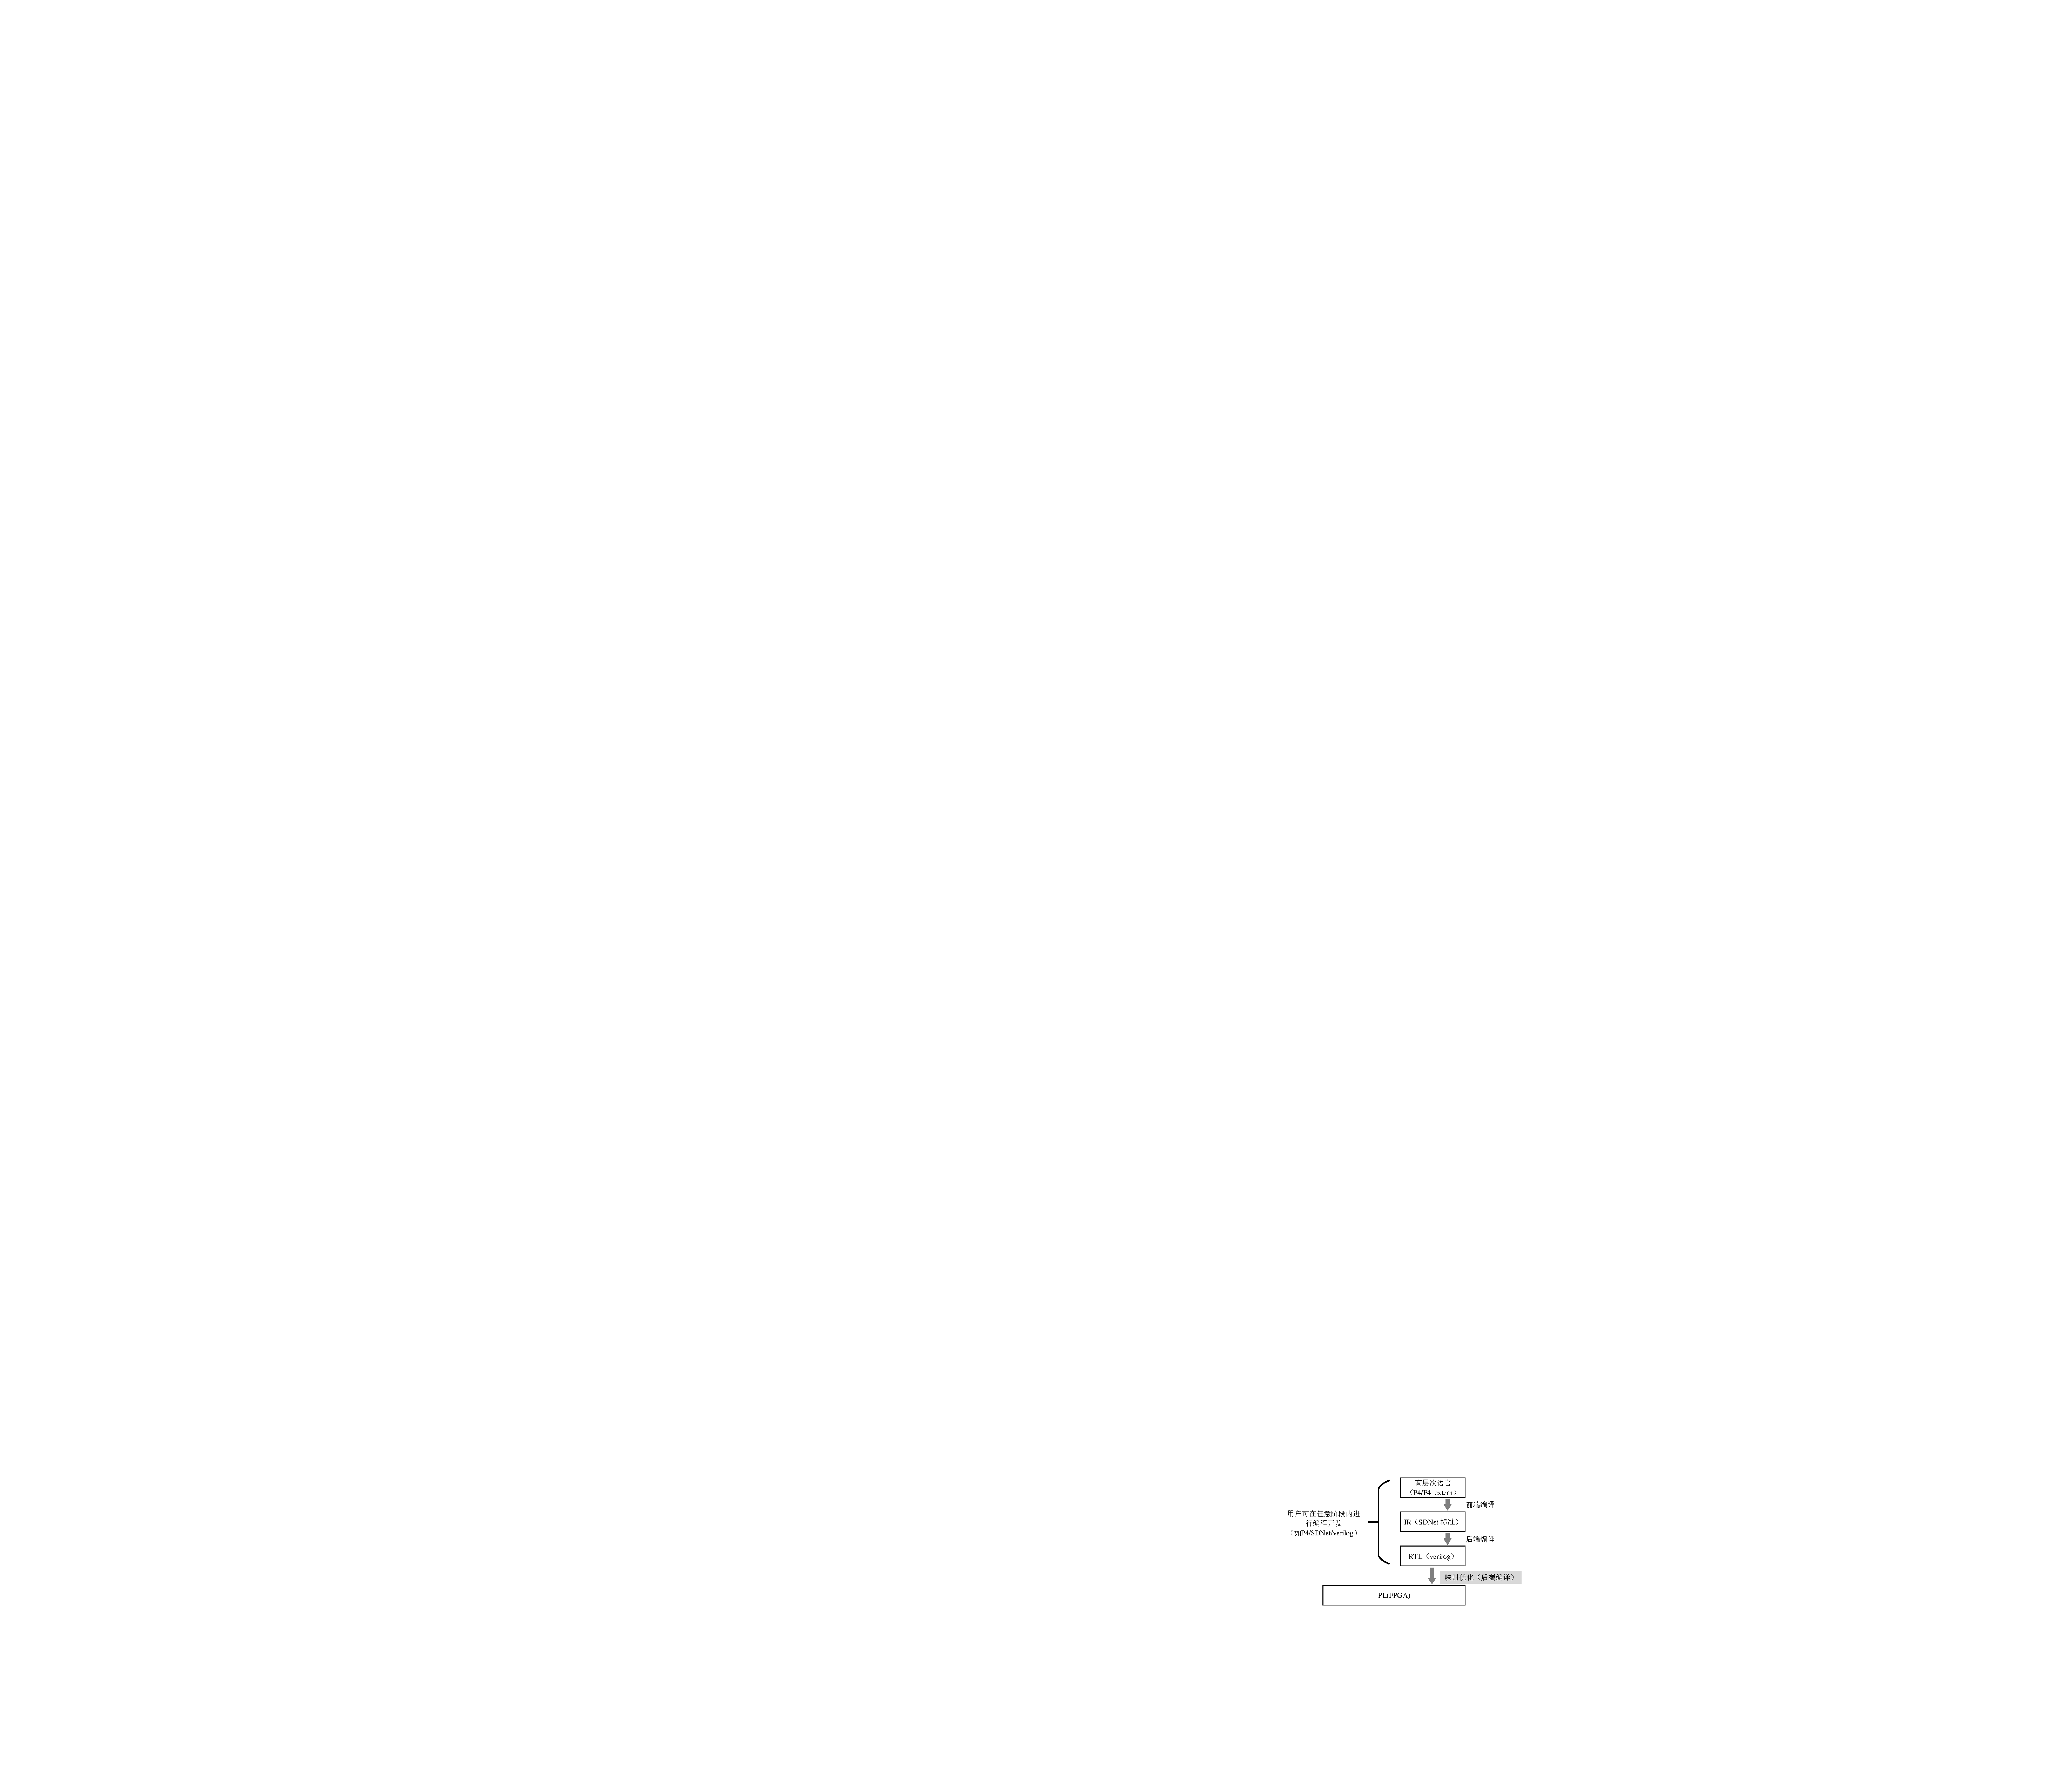
\includegraphics[scale=1]{asdev1.pdf}
	\caption{基于SDNet工具链的FPGA-PL端编译流程} \label{fig:asdev}
\end{figure}

本文利用Xilinx SDNet/P4-SDNet作为建立本文设计原型系统的基本开发工具,基于FPGA的PL编译流程如图\ref{fig:asdev}所示。SDNet和P4-SDNet已经是成熟商用包装解决方案,并包含了为FPGA数据平面设计的P4语言到verilog硬件模块的编译工具链。P4-SDNet内建两种专为P4$ _{16} $(提取包头数据,修改包头域值)提供的P4\_extern功能。这种extern功能给用户提供了足够灵活的直接修改原始数据包头域的能力,但目前此编译器并不支持其他extern对象的编译,且用户也不可定义其自己的extern对象。

使用其类似的思路,本文在开发流程中增加新的编译模块,使其将能够使用户扩展extern对象定义的范围:扩展前端编译器,使其支持其他的高层次描述(描述中增加标记符以提高后端编译器的性能),并将其转译为逻辑中间表示层(IR);最后通过后端编译器再次映射到PL端。
本文提出的硬件转发体系结构与通行产品不同,下面将详细介绍本文开发流程与经典可编程数据平面(以P4为例)之间的差别。

\begin{figure}[!ht]
	\centering 
	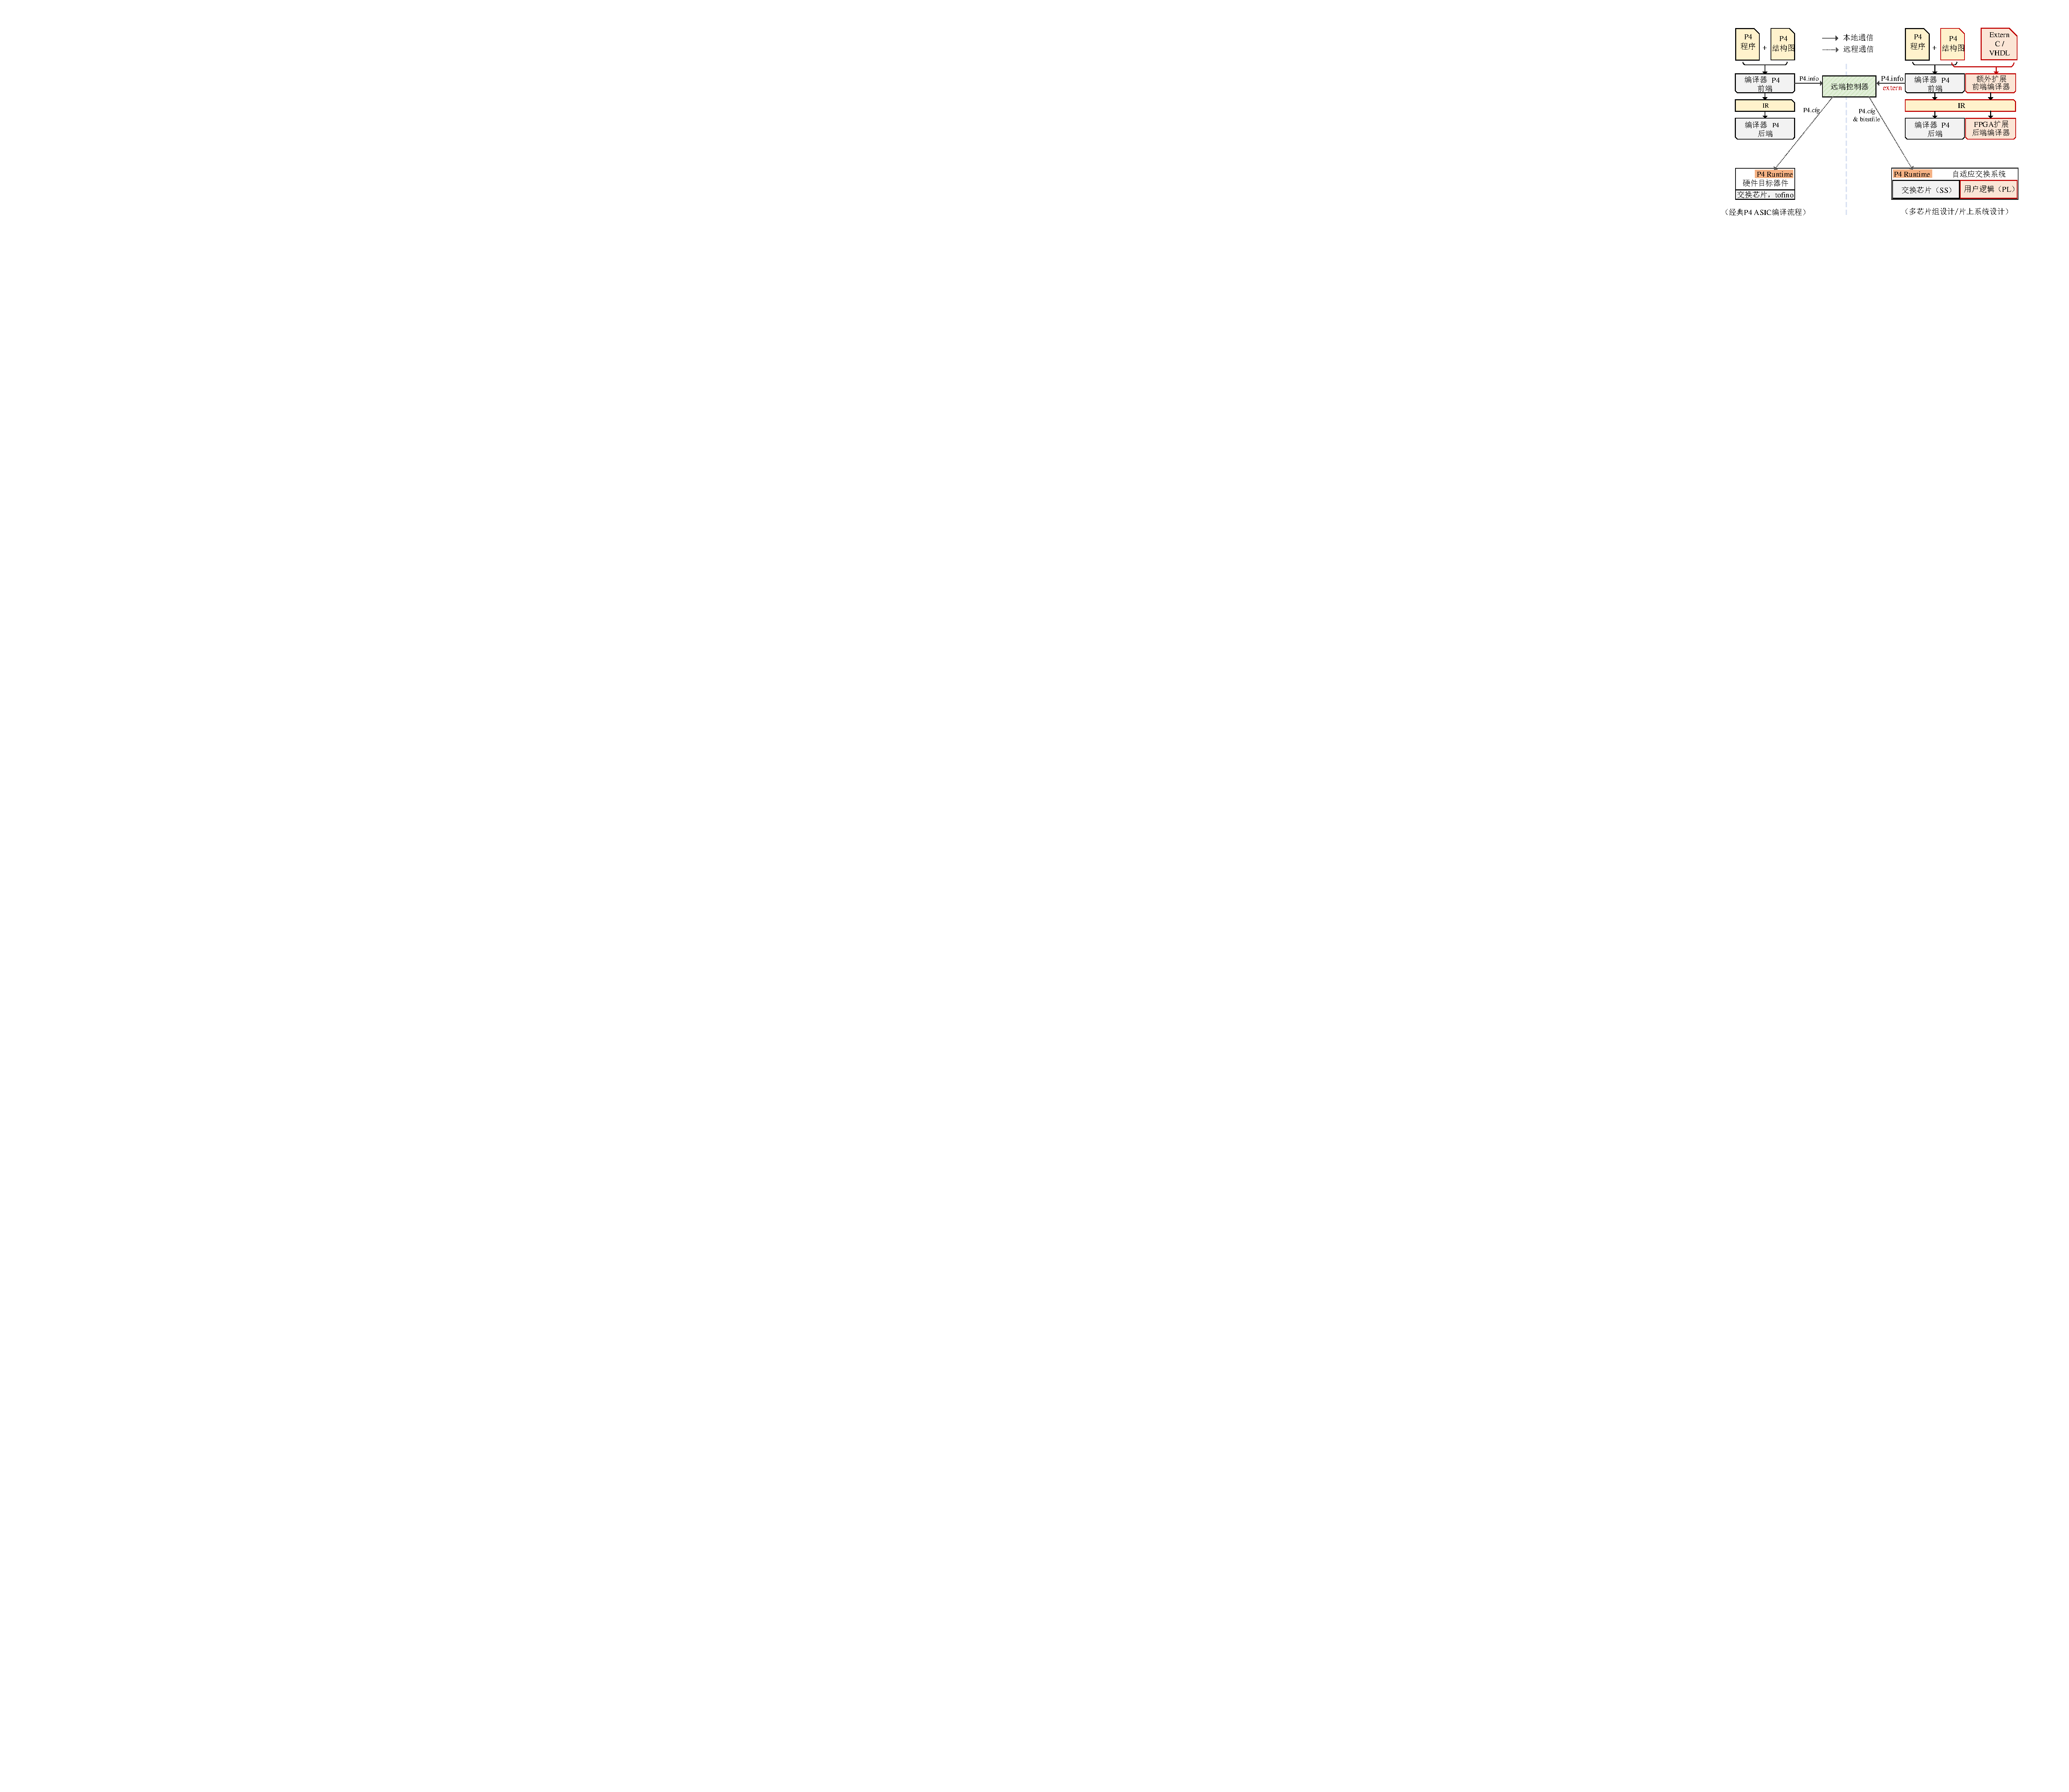
\includegraphics[scale=1]{ascomp.pdf}
	\caption{基于SDNet工具链的FPGA-PL端编译流程} \label{fig:ascomp}
\end{figure}

图\ref{fig:ascomp}中左边为经典的P4程序编译标准流程,对P4目标器件编程需要两个描述文件。首先是P4行为描述程序代码,包含了待处理数据包的包头域定义,包头域匹配关系图,流表设计,执行动作设计等。第二为P4架构图,此文件由设备厂商提供,编译器须根据不同底层芯片实现样式进行有针对性的编译,这样编译器可根据结构图对程序进行等效变换以及重组。前端编译器会将文本代码转换为逻辑关系表,也称作中间表示层(Intermediate Representation, IR),后端编译器一般有厂商提供,可将符合规范的IR表示直接转为机器二级制配置文件。远端控制器将配置文件下载入可编程交换机设备即完成了数据平面重配置过程。此时,控制器也需要收集P4定义信息,以方便后续添加流表项等网络功能设置。

根据之前本文提到的自适应交换系统的额外特点,如图\ref{fig:ascomp}右边所示,本文对基础编译框架进行补充。首先P4结构图需要修改为自适应交换机的底层实现,例如需要体现包头域协同处理机制。其次本文支持高层次语言的PISA\_extern对象编程,因此在额外扩展的前端编译器中,需要将高层次编译器适配入本流程。新增部分由红色区域块所示。最终后端编译器配合P4结构图生成FPGA中的RTL代码,交由FPGA厂商工具链生成二进制流文件(bitfile),通过板上运行时代理下载入FPGA即完成了PL端配置。SS端配置同经典过程所述。

\BiSubsection{高层次语言映射样例}{aa}



{\fontsize{10pt}{0.5\baselineskip}\selectfont
	\begin{lstlisting}[caption={数据平面接口:PL端高层语言描述},label={ascode1}]
	extern extern_example{           				//声明模块名称:extern_example
		ext_type(in bit<wdth> input_Port);			//声明接口位宽以及数据流方向
		int a = VHDL_method_example();				//模块使用其他语言快verilog
		void CPP_HLS_method_example(a);				//模块使用类C的函数描述语言
	}
	control control_example{						//实例化样例模块
		extern_example(0x0) my_extern_example;
		action my_extern_call(){					//调用PL端功能
			my_extern_example.C_HLS_method_example();
		}
	}
	\end{lstlisting}
}

PL以FPGA芯片为例,自适应交换平台可以将SS交换芯片无法完成的用户定义功能映射到FPGA中。用户的额外功能对象须遵循PL端输入输出接口规范。P4语言风格的数据平面接口规范如代码 \ref{ascode1} 所示。代码定义了一个名为“extern\_example”的PL模块,模块可由C语言或HDL风格实现。对外接口位宽以及方向需要标记。在后期可实例化一个或多个样例,每个样例可自由调用PL端模块中的任意描述功能。

{\fontsize{10pt}{0.5\baselineskip}\selectfont
	\begin{lstlisting}[caption={extern实例的C++类声明},label={ascode2}]
	#include <hls/hls_sim/extern.h>					//头文件extern.h 定义了外围数据传输
	using namespace std;
	template <typename .. Args>
	using ActionPrimitive =
		hls :: ActionPrimitive <Args ...>;
	using hls :: Data;
	class extern_example: public ExternType{
		public:
			void init() override{}
			void C_HLS_method_example(){...}
	};
	HLS_REGISTER_EXTERN(extern_example);
	int import_extern_example(){return 0;}
	\end{lstlisting}
}

如代码 \ref{ascode2} 展示了C++风格extern函数。头文件“extern.h”中定义了核心函数之前的流水线结构(需要用户注意并修改),无需提现在核心描述代码中。FPGA高层次编译工具链(SDx,Bluespec System Verilog)可读取此类文件,并综合成带有用户功能的IP核,小的IP核可便于集成进更大的FPGA工程。

{\fontsize{10pt}{0.5\baselineskip}\selectfont
	\begin{lstlisting}[caption={extern实例的VHDL模块声明},label={ascode3}]
	`timescale 1ns/1ps
	module VHDL_method_example#(
		parameter DATA_WIDTH = D_WIDTH,
		parameter CTRL_WIDTH = C_WIDTH,
		parameter EXTERN_REG_WIDTH = R_WIDTH,
		...
		)(//---data interface
			input		[DATA_WIDTH - 1:0]	in_data,
		  //---register interface
		  	input [EXTERN_REG_WIDTH - 1:0]  in_reg,
		  //---misc
		  	input							clk,
		  	input							reset);
		  	
		//local parameter
		//wires/regs
		//modules
		//method example logic
	endmodule //VHDL_method_example
	\end{lstlisting}
}

代码 \ref{ascode3}展示了VHDL语言实现PL实例模块,在VHDL中须描述数据总线位宽,寄存器通路接口等。对于其他硬件系统,用户只需要指定通信用同步数据总线的时钟周期(时间约束)。
实际上,本文所描述的所有编译工具链仍处于设计阶段,并需要大量代码工作完成自动化处理。本文主要目的在于规划框架以及作为商用工具链的补充设计参考。硬件开发时间周期过长,为快速进行数据平面验证,本文生成的所有bit文件均为手动整合代码。

\BiSection{硬件设计}{aa}

\BiSubsection{协议设计}{aa}

\begin{figure}[!ht]
	\centering 
	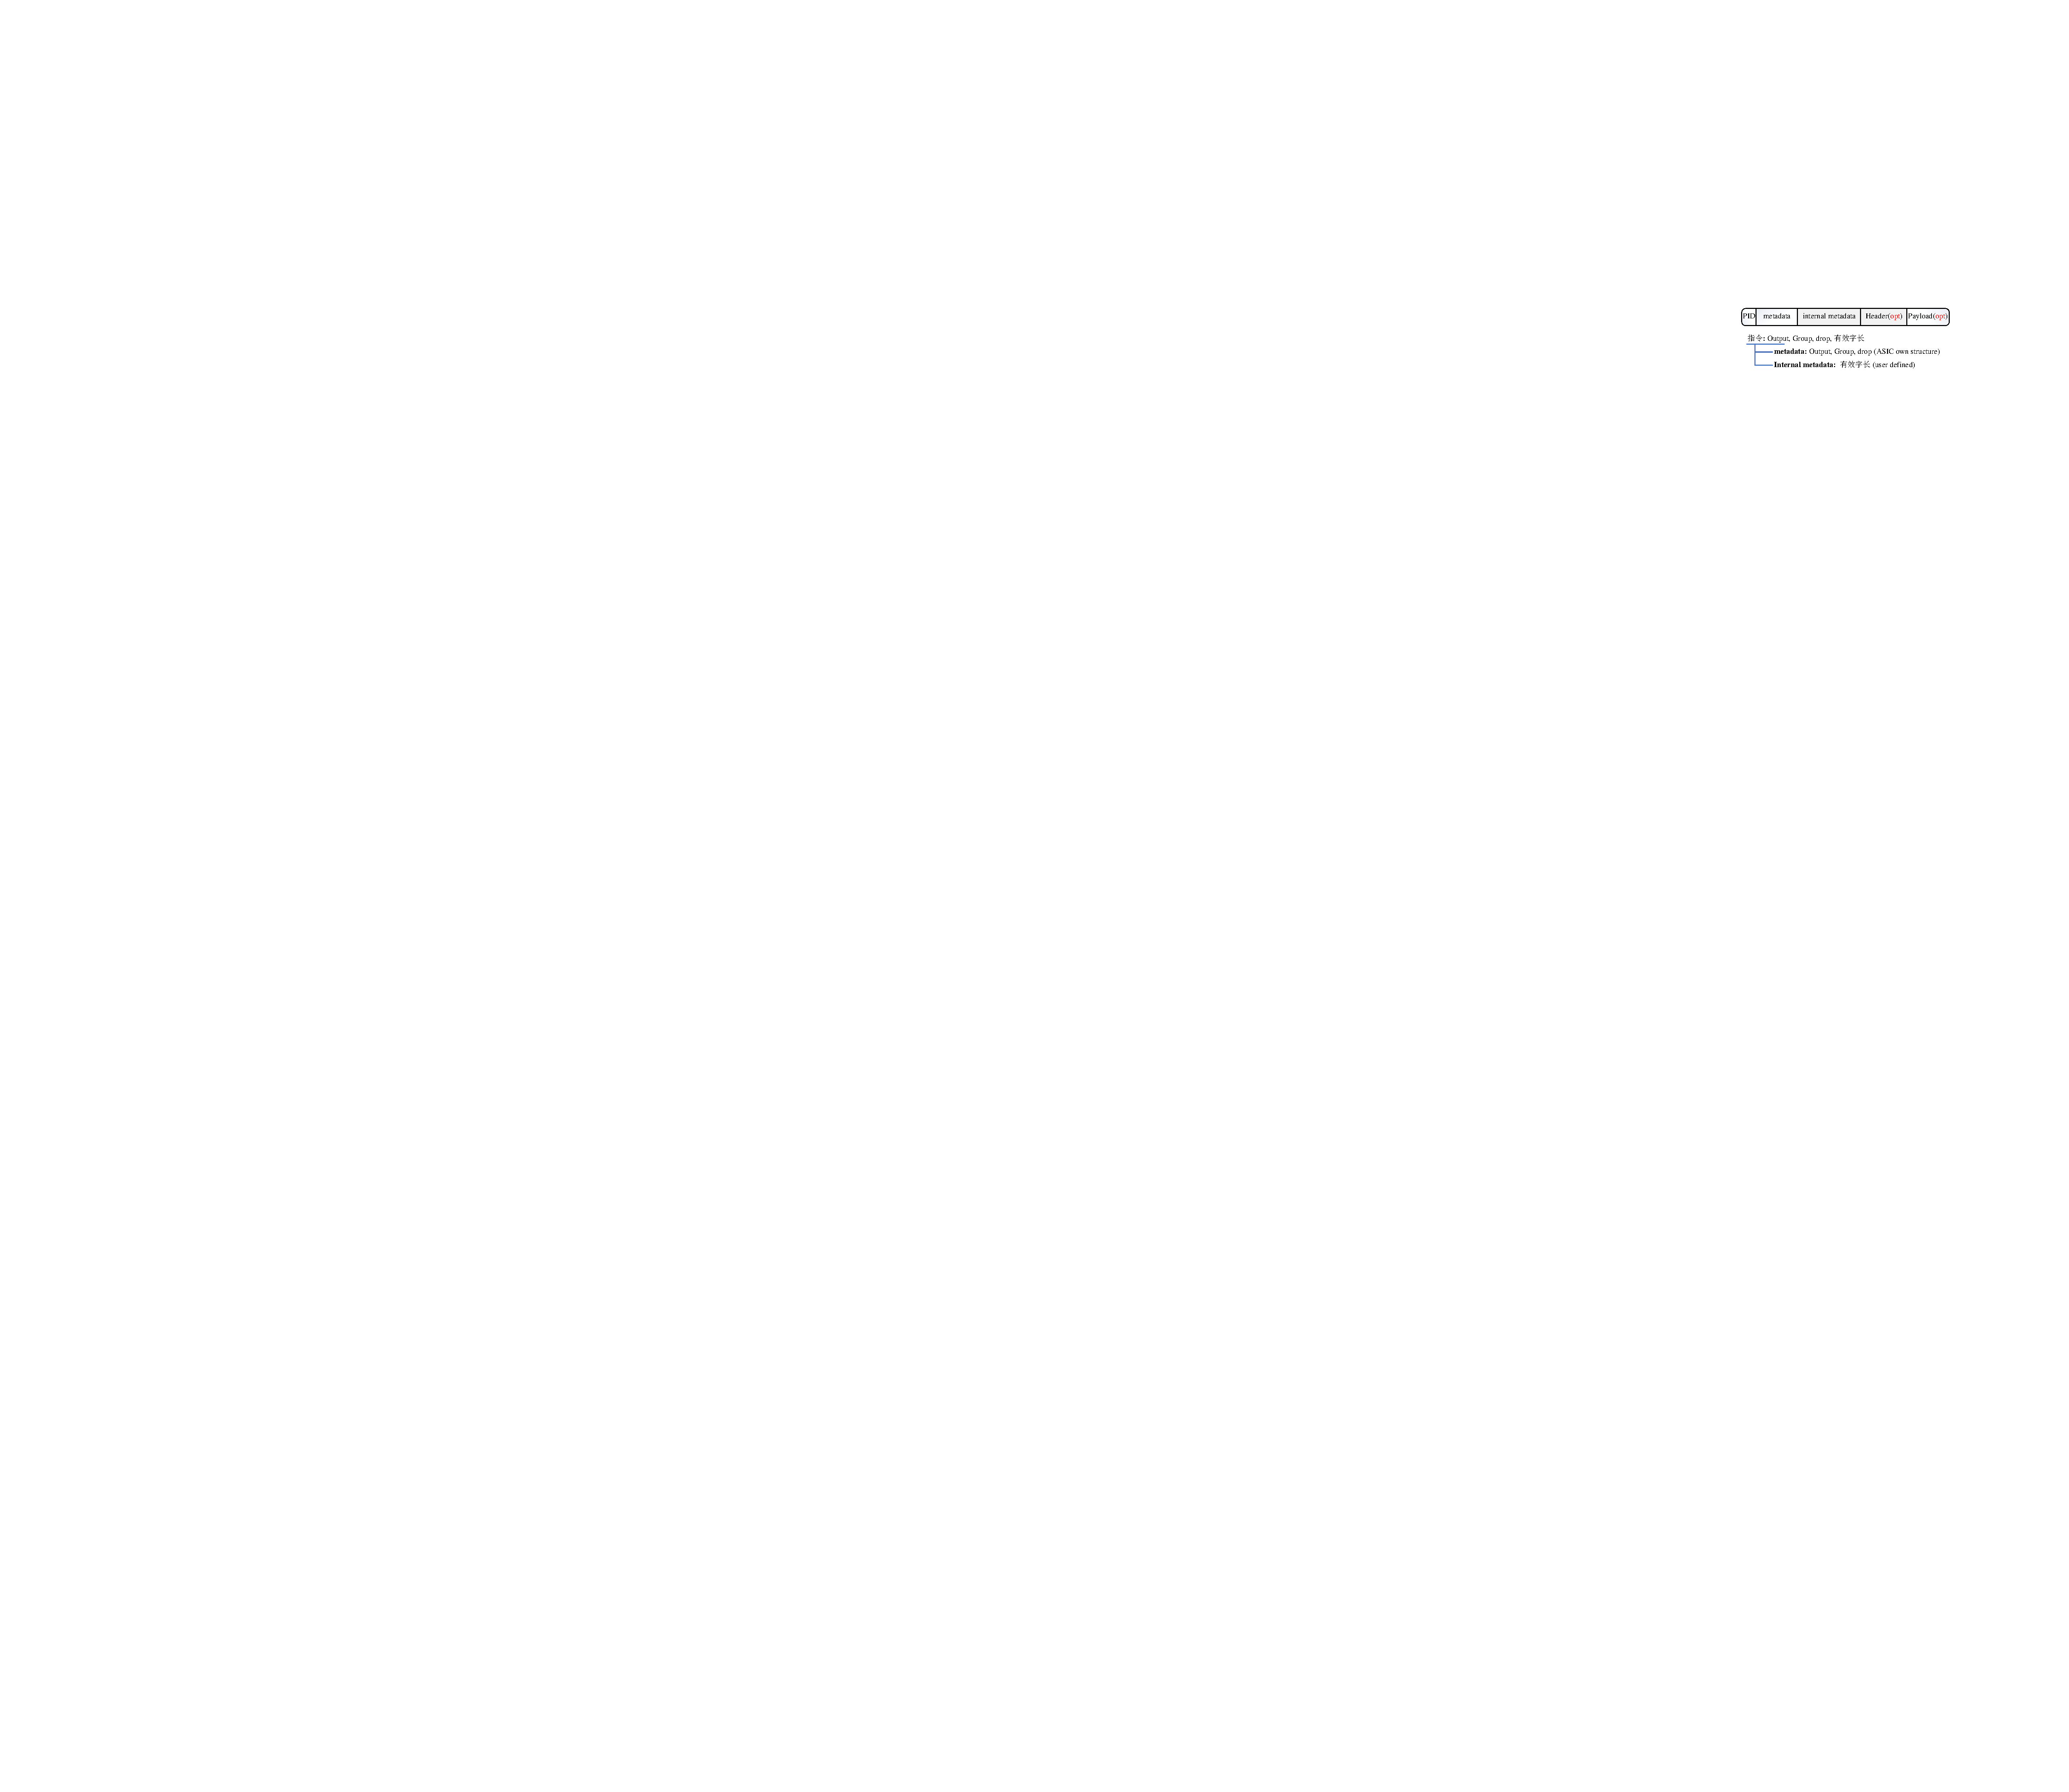
\includegraphics[scale=1]{asframe.pdf}
	\caption{SS与PL内部通信帧格式} \label{fig:asframe}
\end{figure}

上节提到自适应交换架构中SS端与PL端的通信须包含元祖数据以及包头,本节论文详细讨论通信帧格式。本文设计了一种通信帧(可满足大部分需求,用户也可以自行定义),格式如图\ref{fig:asframe}所示。首先帧头指定了帧的编号PID,帧由SS中的数据包生成,完整的数据包与帧使用同一个PID编号,方便PL协处理器处理之后重新组合。元祖信息(metadata)包括了数据包转发过程中的信息,例如输出端口,组表编号,丢包等。用户元组信息为帧有效字长,由于用户可以定义帧长度,这将给用户极大的灵活性空间。此外用户还可定义包头长度以及携带的数据包负载信息长度等。SS与PL之间传递的大部分操作数都是商用ASIC中已经实现的指令,因此SS端设计可以极大程度复用已有芯片设计。须增加的功能只有帧长度信息等域,这样可使对ASIC改动降到最低。

\BiSubsection{SS端固定功能}{aa}

SS端对于目前商用普通交换芯片中需增加的功能为第一小节中提到的图 \ref{fig:asarch}内左边虚线内的MMU模块。自适应交换的核心思想是利用基于ASIC的交换系统(SS)提供包交换的高性能,而用可编程硬件协处理器(PL)提供包处理的灵活性。因此在SS端本文将包处理逻辑做的最简化,只保留一个用户可配置逻辑(即帧长度的定义)。MMU将用户定义的不超过帧长度的包头数据(指某一区间段)复制到通信帧中即可。MMU的其余工作还包括了动态申请和释放数据包缓存空间,以及重组数据包。接下来本小结主要介绍MMU的分析与设计。

假设SS与PL之间单向通信带宽有256G(PCIe4.0),以帧内包含完整64字包头节为例,则包速率达到380Mpps。目前交换芯片的时钟驱动频率大约在1GHz到1.5GHz之间。对于MMU模块,若留给每个数据包的处理时间3周期则不会超过时钟频率(需要约1.2GHz主频)。在之前的MMU设计中,内存被分割为每页256字节。调度器以页为单位进行分配,维护逻辑映射与物理映射之间的关系由于页容量比较小而变得比较复杂。因此MMU瓶颈处理一个分配任务需要耗时25周期\citeup{wang2017p4fpga},尽管这种设计思路在资源利用率上比较占优(平均资源浪费仅为1/2page),但它的时间复杂度太高,导致分配性能受影响。在ASIC的存储设计中,其经济性要好于由FPGA组成的片上存储资源。因而本文在设计存储单位时将每个地址对应的容量配额扩大为1.6KB(可完整放下一个最大包)。在分配以及查找长包时,可节省逻辑地址与物理地址之间多次正向/反向映射过程,因此大大提升分配速度。

\begin{figure}[!ht]
	\centering 
	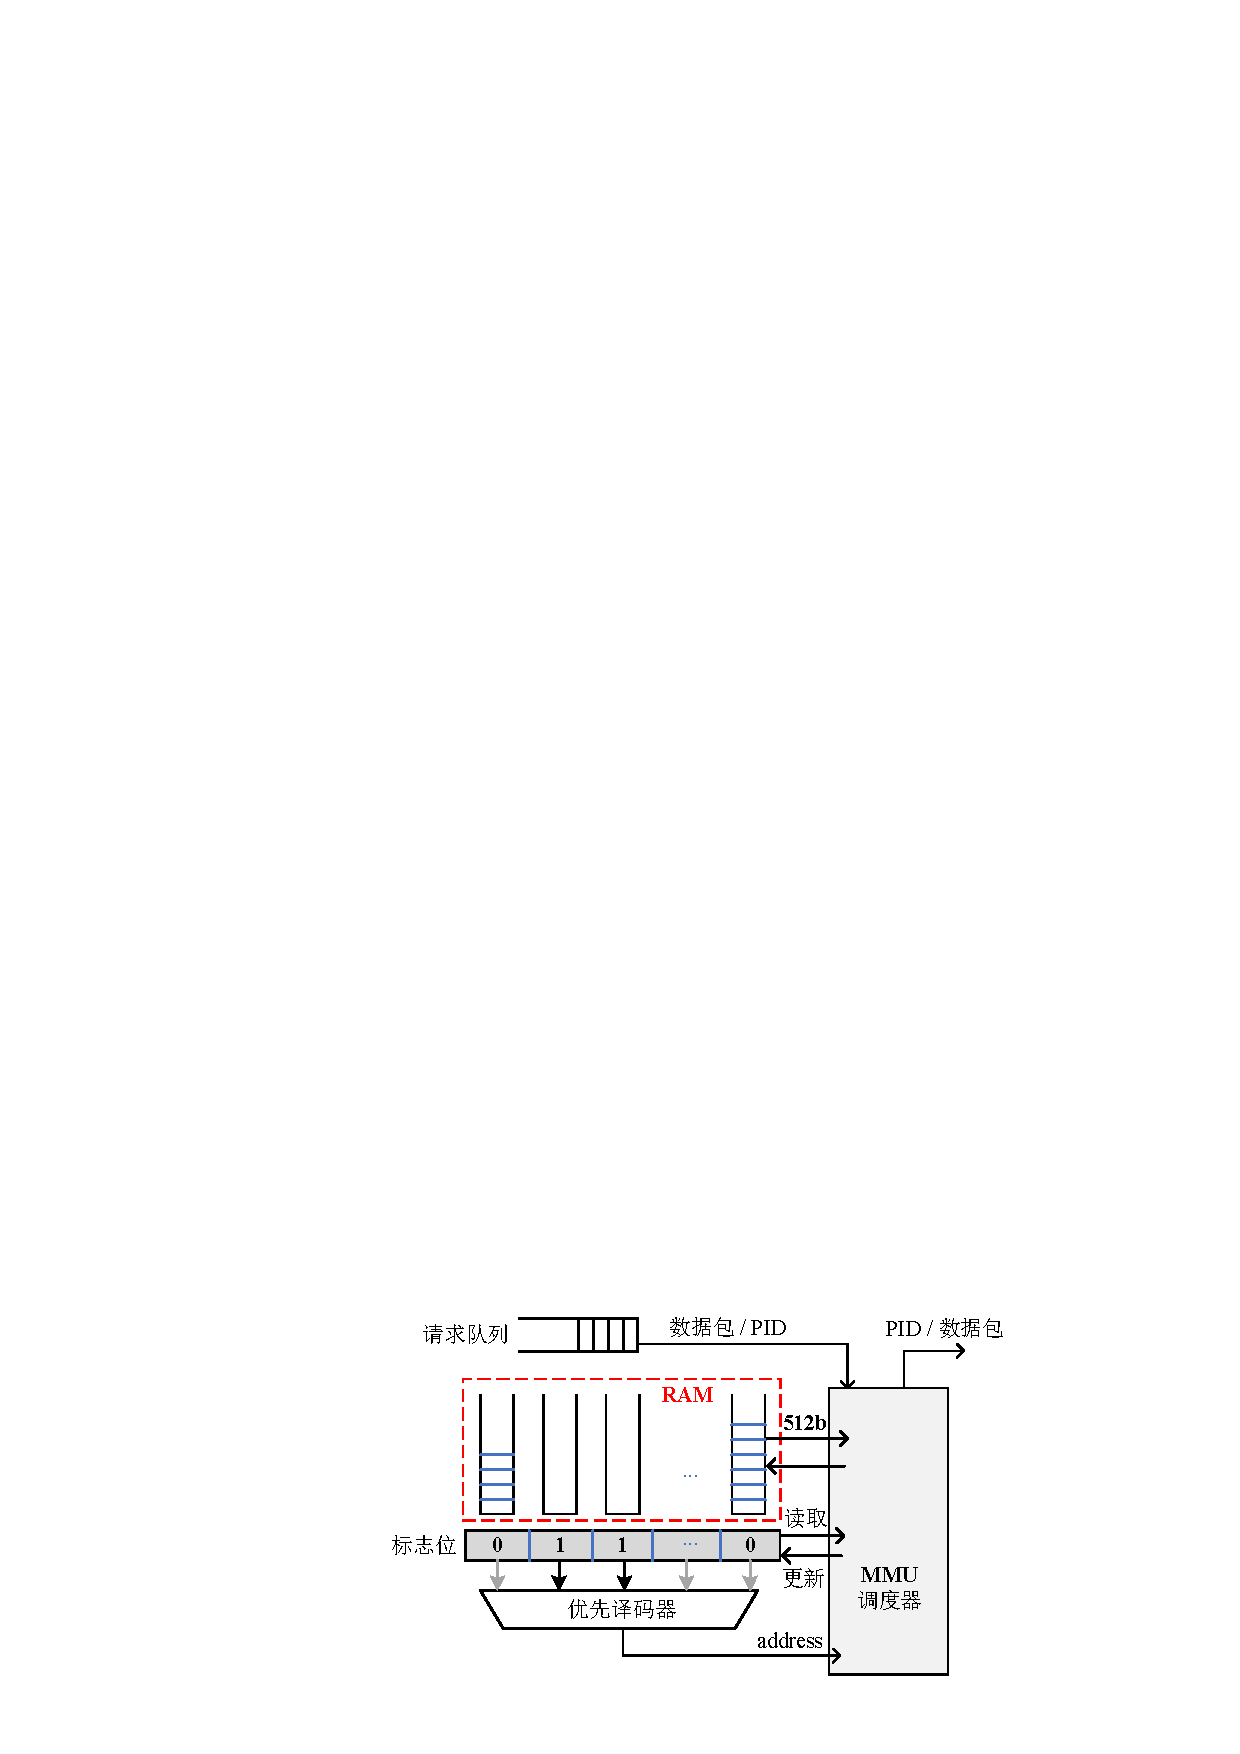
\includegraphics[scale=1]{asmmu.pdf}
	\caption{高pps性能MMU的实现方案} \label{fig:asmmu}
\end{figure}

如图\ref{fig:asmmu}所示,本文使用了一组“标志位”寄存器来指示其对应的page空间是否被占用。当数据包请求一个新的可用地址时,优先译码器会将标志位最左边为“1”的位置作为地址(address)返回给调度器,且便立即将此位置的标志“1”更新为“0”。之后调度器会把数据包向此位置写入,并且令此位置的地址作为PID值填入PL通信帧的首部。当MMU收到一个含有PID值的读请求时,MMU会读取以PID值为位置的存储空间并将其组合为数据包重新发出到入队流水线中,完成后立即将此位置的标志位为“1”。此时数据包的metadata中一般包含了由PL端处理完成给出的执行需求,SS端无需对此包做额外的分析工作。为了防止地址冲突以及标记位数据不同步带来的读写错误,优先译码器必须在完成上一个“读/写”请求之前,更新空闲地址,以备调度器无缝衔接下一个写请求,读请求则无需使用优先译码器结果,无操作风险。上文分析过,对每个读写操作,MMU都预留了3个时钟周期的处理时间。在系统运行后,由于数据包连续到达以及连续读写,因此在一段时间内,平均读次数是等于写次数的。MMU将读写交替进行,可为写请求争取6个时钟周期的译码时间,一般来讲对于有4k个位置的优先译码器,6个时钟周期足够通过硬件并行地两两比较找出最优位置(每周期比较两次的情况下$2^{6\times2}=4096$,但一般可以比较次数更多)。

接下来分析MMU应维护的内存容量大小。在元祖信息帧由PL返回之前,数据包都需要维持在MMU的存储空间内。假设信息帧处理时间为$T=n$((微秒),上文提到总体包处理频率不超过$v=$380Mpps,因而平均在等待的数据包个数为$T \times v \leq =380n$。目前板间硬件处理时延应保证在3微秒以下,如果使用片内AXI总线互联,则完整处理时间应保证在1微秒\citeup{xilinxpcie}以内\footnote{在数据包的处理过程中查找TCAM表是最费时间的,一般需要20个时钟周期,但正常处理流程内TCAM表项不会超过2个。普通精确匹配查找表只需要不超过3个时钟周期即可。我们假设比较悲观的情形,PL内的处理过程包含5级TCAM查表以及10级精确匹配查表,则总共须耗费650时钟周期。若以200MHz主频运行FPGA,则总耗时约0.7微秒(一般只需要0.1微秒)。因此本文认为,PL的处理时延主要由信息帧传输过程贡献。PCIe收发器结构复杂,突发的批次传输时延较大(100时钟周期\citeup{xilinxpcie}),但高性能片上AXI总线的传输时延也很低(不超过10时钟周期)。}。为保险起见,本文将处理时间余量增大十倍假设最大不超过10微秒,则根据上式,可约估SS端等待数据包个数为4k个。上文提到每个数据包存储位置占用1.6KB,则板上共计须设置最多为6.4MB存储空间。以目前的半导体工业水平可满足此需求。 



\BiSubsection{PL设计}{aa}

基于FPGA的PL设计最大的挑战来自于大批量信息帧的处理速度(380Mpps)。对于PL内部逻辑,由于帧内包含了基本的metadata信息以及包头域段落,对PL的性能设计可将其按照网络处理最小包(64字节)的方式分析。按照FPGA主频200MHz计算,即使每个时钟周期都能由流水线处理完成一个数据包,FPGA的性能也只能达到200Mpps。对于某些带状态阻塞性处理机制(如有状态查找表),平均需要2-3个时钟周期才可处理完成一个数据包,因此FPGA的处理性能会下降到60Mpps。远远达不到系统设计的需求。

一种思路是将FPGA内一条流水线完整复制多份,以均分总体任务量。例如可以将流水线同时复制$K$份,平均总处理性能是每条子流水线的$K$倍。然而这也意味着总资源提供量需要耗费之前每条流水线的$K$ 倍。但由于数据包流水线内有查表等大资源消耗量组件(1k深度的TCAM表项可占据整个FPGA逻辑资源的1/3),有限的FPGA逻辑面积不可能满足多条并行流水线的资源占用需求。

为解决上述挑战,本文提出一种微结构并行数据包处理流水线设计(micro-level parallel processing)。微结构流水线的核心思想是将原有的大表项拆分为多个小表项的等价组合,即通过不完整的复制大资源模块,而满足原始用户语义下的数据包处理需求。总结如下,本文将通过以下两个关键技术解决高效PL处理设计,1)提出一种资源高效的并行数据包处理架构,2)通过流表编译算法将流表项映射到多路子流表中,以达到流量均衡并高效利用硬件资源。

1)资源与性能

查找表是数据包处理过程中最核心的部件,也是资源消耗最大的组件。为提升效率本文需要依靠并行子流水线的思路扩展数据包处理性能。同时,为满足资源消耗限制的约束,本文需要分析如何拆分流表。另外,多级流表是目前交换系统中流水线的重要设计特征。多级流表可以降低单张表的资源消耗,但每条子流水线中只包含部分信息,无法保证同一条流水线内数据包的完整处理诉求。 




2)并行流水

流水线被分为$K$个并行子流水线后,数据包流也应被尽量平均地分类为$K$份。然后将不同的组份以流量均衡的形式放置在不同的子流水线中。本文将数据包按照包头信息内的ID比特位来分成$j (j > K)$个组份。例如,将包头信息哈希为$n$ bits数值,以此数值来代表不同的流组份(根据哈希函数定义,同一条流的所有数据包均可分到同一个组份),则共可分成$j=2^{n}$份,显然每一份的流量大小是不一定相等的。如图\ref{fig:pljidk}所示,本文将j个ID组份以流量均衡的形式安置在K条不同的流水线中。

\begin{figure}[!ht]
	\centering 
	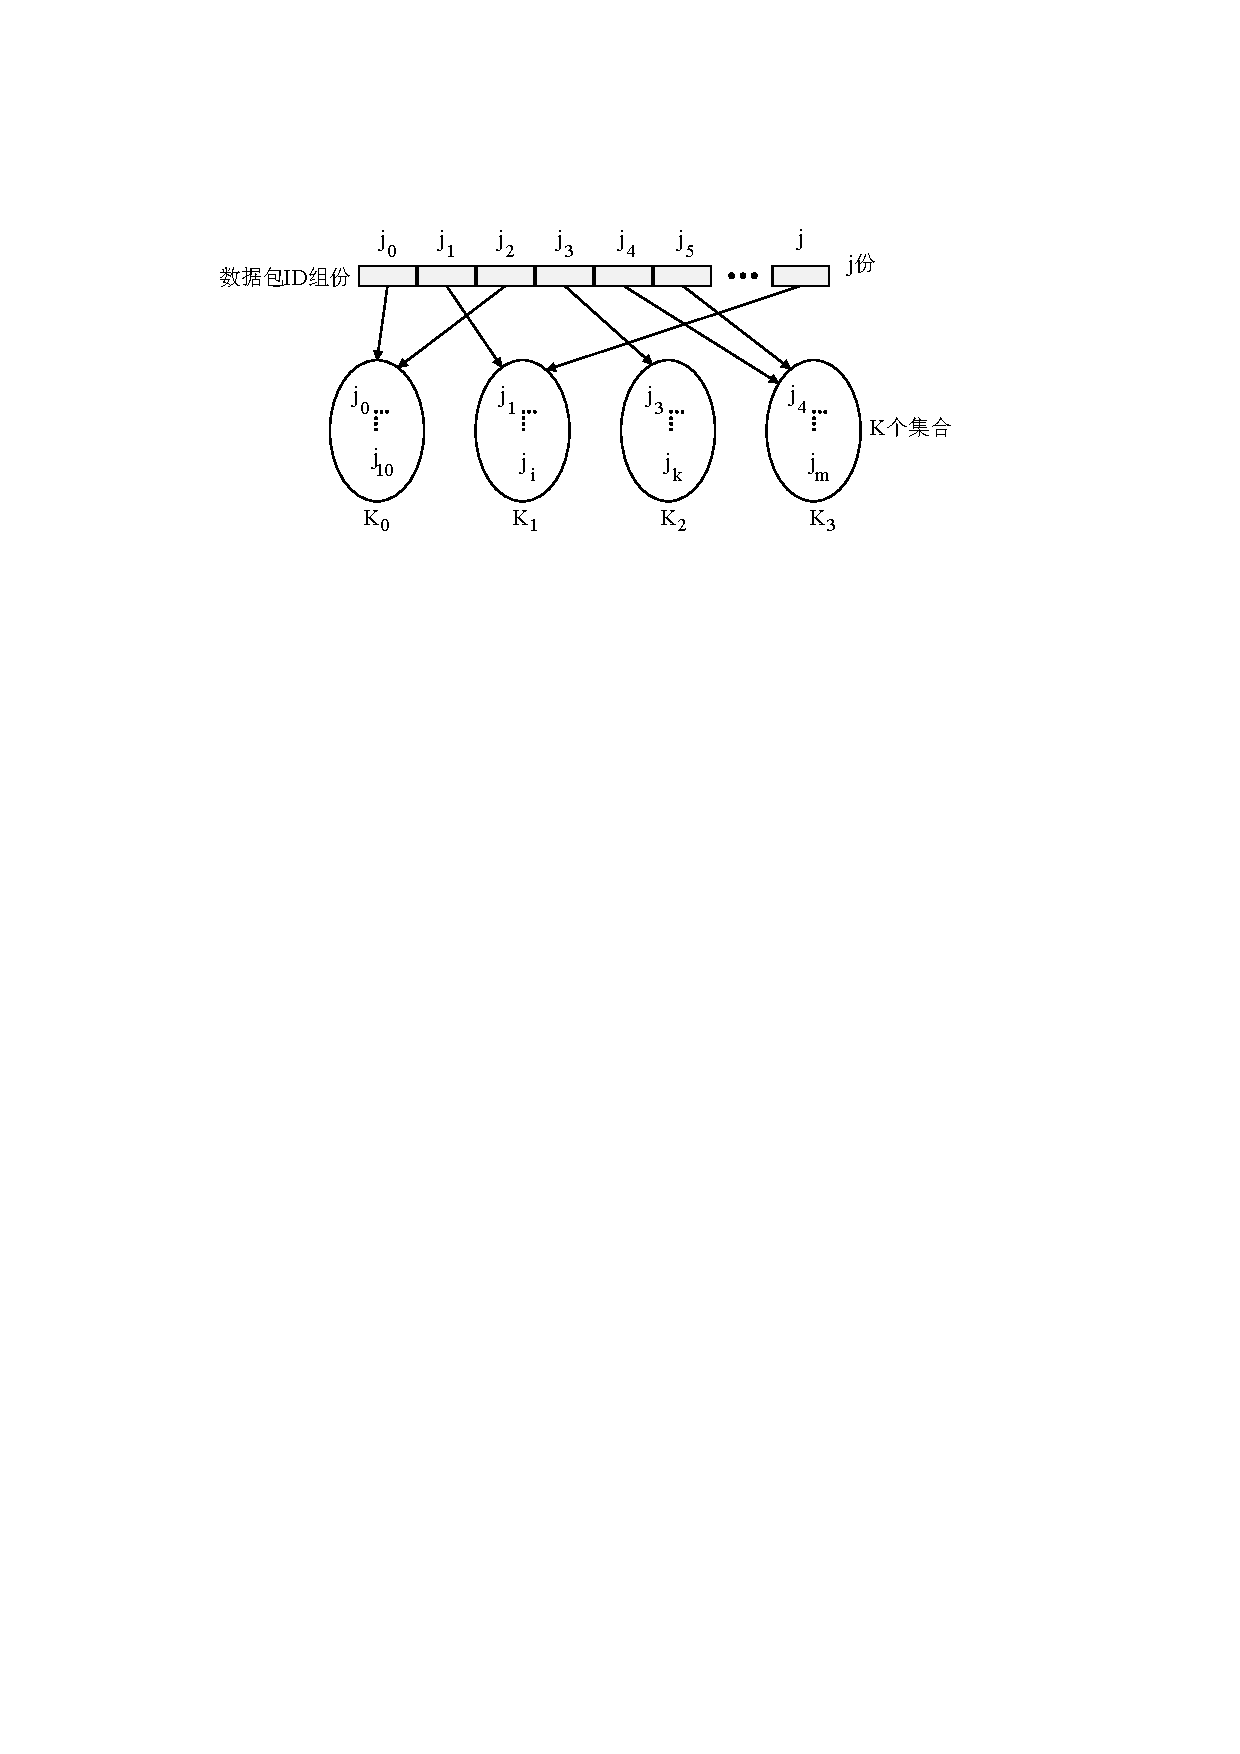
\includegraphics[scale=1]{pljidk.pdf}
	\caption{$ j $组ID组份向$ K $个集合中分配} \label{fig:pljidk}
\end{figure}

为确保每个$K$集合中流量均衡,可调整$j_i$的排列,若假设$ j_i $为第i个组份的流量大小,使得每个集合之间的总流量大小相近。则集合总流量$ K $可表示为:

\begin{equation} \label{pl1}
K_0=\sum_{i_0}^{k_0}j_{i_0}
\end{equation}

3)流表拆分

本文首先讨论在PL端不同类型的流表拆分原则,然后讨论如何使拆分表组合为多级流表之后的语义保持不变。查找表从功能以及实现方式可以分为精确匹配和掩码匹配。由绪论部分可知,精确匹配目前有两种实现方式:(1)内容地址映射表(CAM),(2)基于RAM的查找表;掩码匹配可由TCAM实现。

前文提到,数据包在进入子流水线之前须经过哈希函数(hash())分类,并确定最终去往的目标子流水线。将流水线分为$K$份,则流表也需要拆分为$K$份。哈希函数将全体数据包流分为了$j$份,因此利用哈希函数也可以将流表内容分为$j$份,并按照集合$K$中的分布,将流组份$j$对应的所有流表项也分配到$K$个流水线中。下面依次介绍每种表的拆分方法:

\begin{itemize}
	\item CAM表。此过程对于精确匹配的CAM表的分类比较直观,只需要按照哈希结果,将CAM表中每一条流表项分到对应的K集合内,亦可保证语义正确。
	
	\item LPM(Longest Prefix Matching,最长前缀匹配)表。与CAM不同,PLM表内含有掩码位(*)。不同的数据流被哈希函数分到不同的组份,由于不同的组份有可能被分到不同的子流水线,有可能导致被同一条LPM表项同时匹配的两条流被分到不同的子流水线。若按照无复制方式去拆分流表项,则必然造成一部分流量无法匹配成功。如图\ref{fig:plmask}所示,在做流量分类时,选取包头域中四个bit位进行哈希取值。若这些bit位中有位置对应到了带掩码表项(1*10),而此时,两条流“1010”与“1110”恰好又被哈希函数分到了两个子流水线中的组份($j_1$与$j_2$),则此掩码表项须分别复制到两条子流水线中。
	\begin{figure}[!ht]
		\centering 
		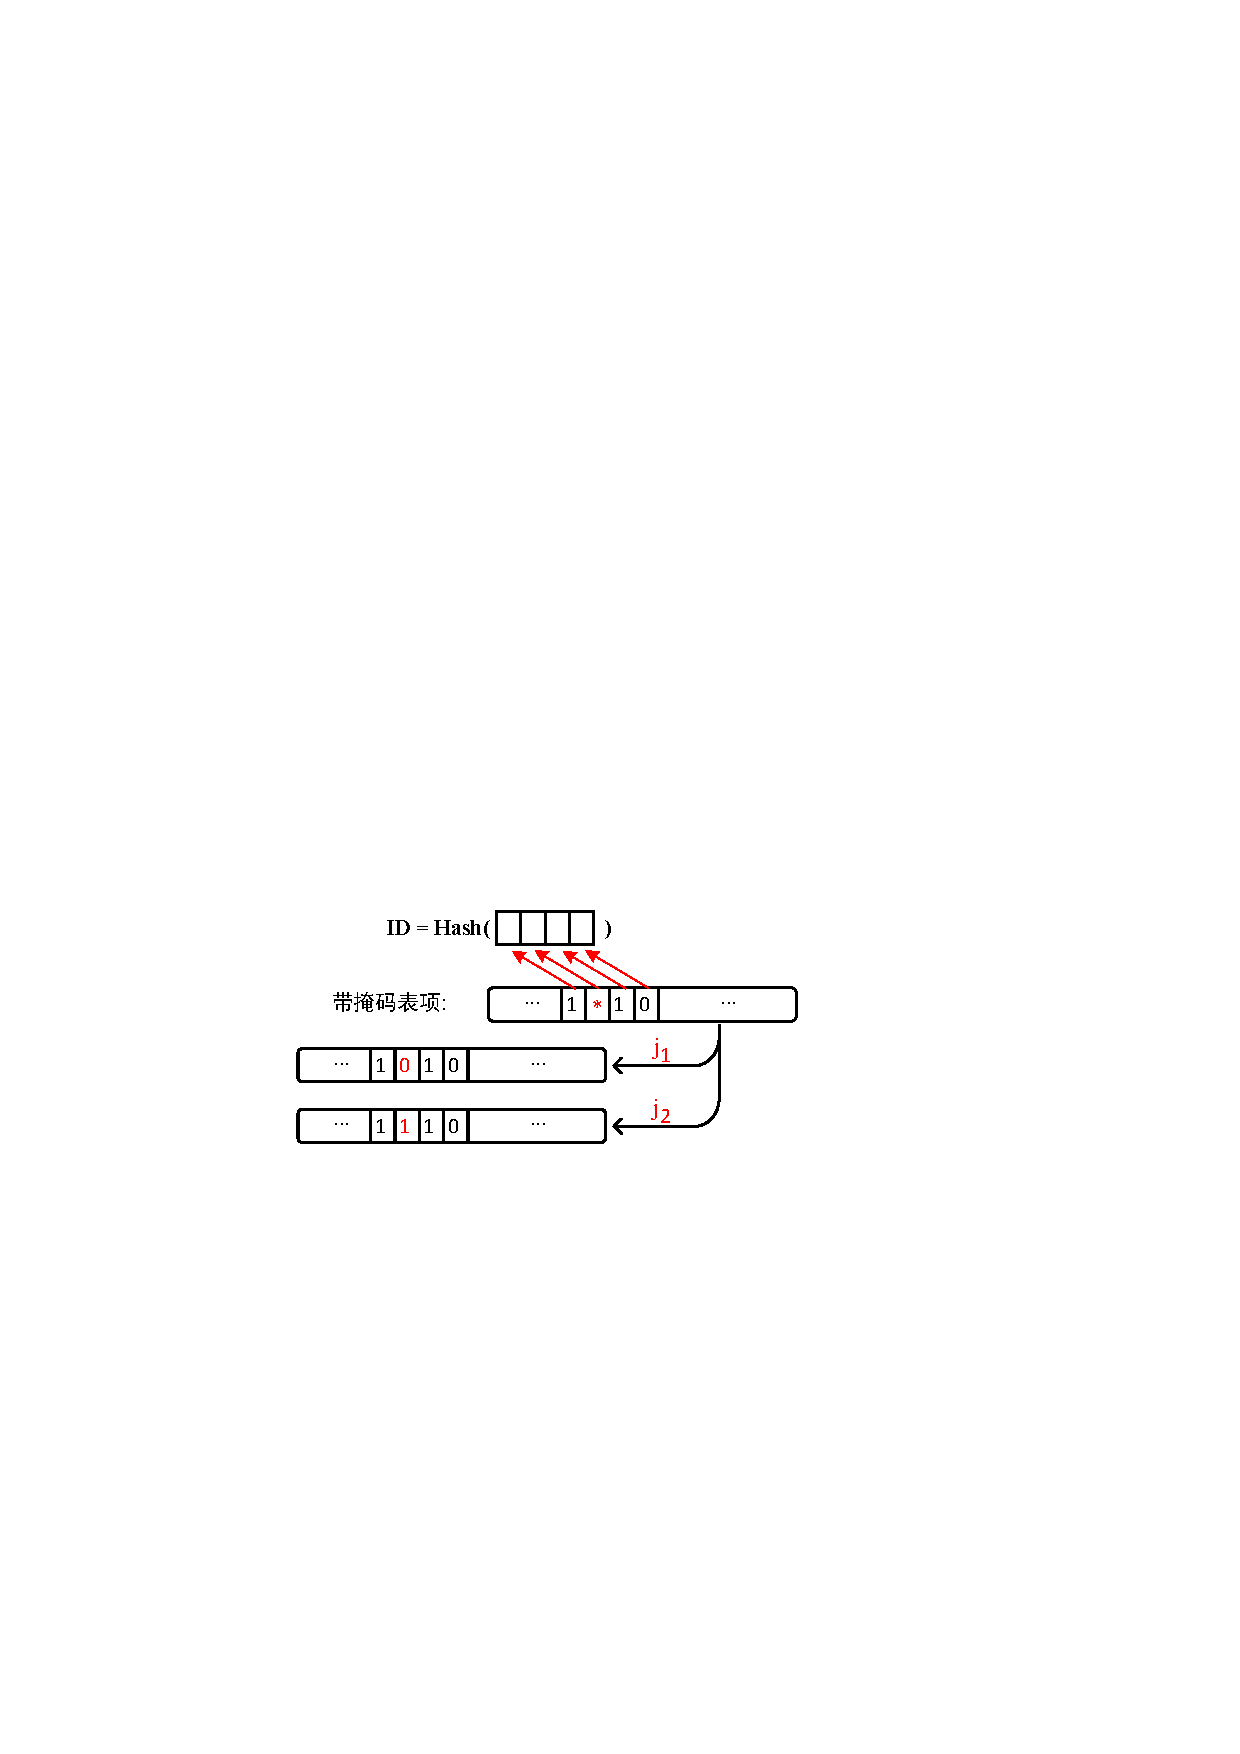
\includegraphics[scale=1]{plmask.pdf}
		\caption{带掩码表项在拆分时,可能需要被复制多份} \label{fig:plmask}
	\end{figure}
	\\因此带有掩码的表项在做并行子流水线拆分时会占用比拆分前更多的表项空间。例如在IP路由查找场景下,通过分析掩码的位置以及流组成发现\citeup{zheng2006tcam},适当调整包头域中抽取的bit位作为哈希函数的输入值,可保证多占用的表项空间维持在比较低的水平(6\%左右)。因为如果不选择带有掩码位置的bit为作为输入,则可化简为精确匹配的场景,因此也不会遇到无法匹配的问题。
	\item TCAM表。与LPM相似,根据哈希函数抽取bit位置是否带有掩码(*)位,TCAM表项也可能会占用比原始表项空间更多的流表项数目。
	\item RAM(直接查找)表。查表时以带搜索KEY的值为地址,直接读出RAM地址位对应的存储数据作为搜索结果。若搜索的数据位宽为$ KEY $位,则RAM表的深度应为$2^{KEY}$。由于RAM表的深度只与KEY的位宽相关,RAM表的存储依赖于连续地址空间,因此RAM表拆为$ K $个也无法使RAM表的容量缩小为原来的$1/K$。在第二章本文介绍过,由于使用RAM查表的域宽度一般不大,只有16位(查找端口号等),占用空间很小(不超过总资源的0.5\%),可以考虑完整复制。其次,若RAM真实利用量比较小,可以用CAM代替RAM表,从而更节约逻辑资源。
\end{itemize}

4)多级流表与流量均衡分类器

在数据包处理的过程中,假设匹配N个域,每个域共M个流表项,若只使用一张流表,则总共需要消耗$ M^N $深度的流表项。一般实际应用时,会为每个域单独设立一个查找表,多个域使用多级查找表以串行流水线方式完成匹配过程。这样只需使用$M\times N$深度的表项,可大大节约资源消耗量。

然而,通过第一条子流水线的数据包在匹配下一个域时,下一张流表的流表项不一定与此数据包处于同一条子流水线。如图\ref{fig:pllb0}所示,数据包p0根据流量均衡哈希函数被分配到第1条子流水线,经流表0匹配结束后,此数据包还需流表1继续匹配,但此时发现,处理p0数据包对应的流表1不一定依然存储在流水线1中,也许被拆分到了流水线K-1内。则数据包p0无法得到后续服务。

\begin{figure}[!ht]
	\centering 
	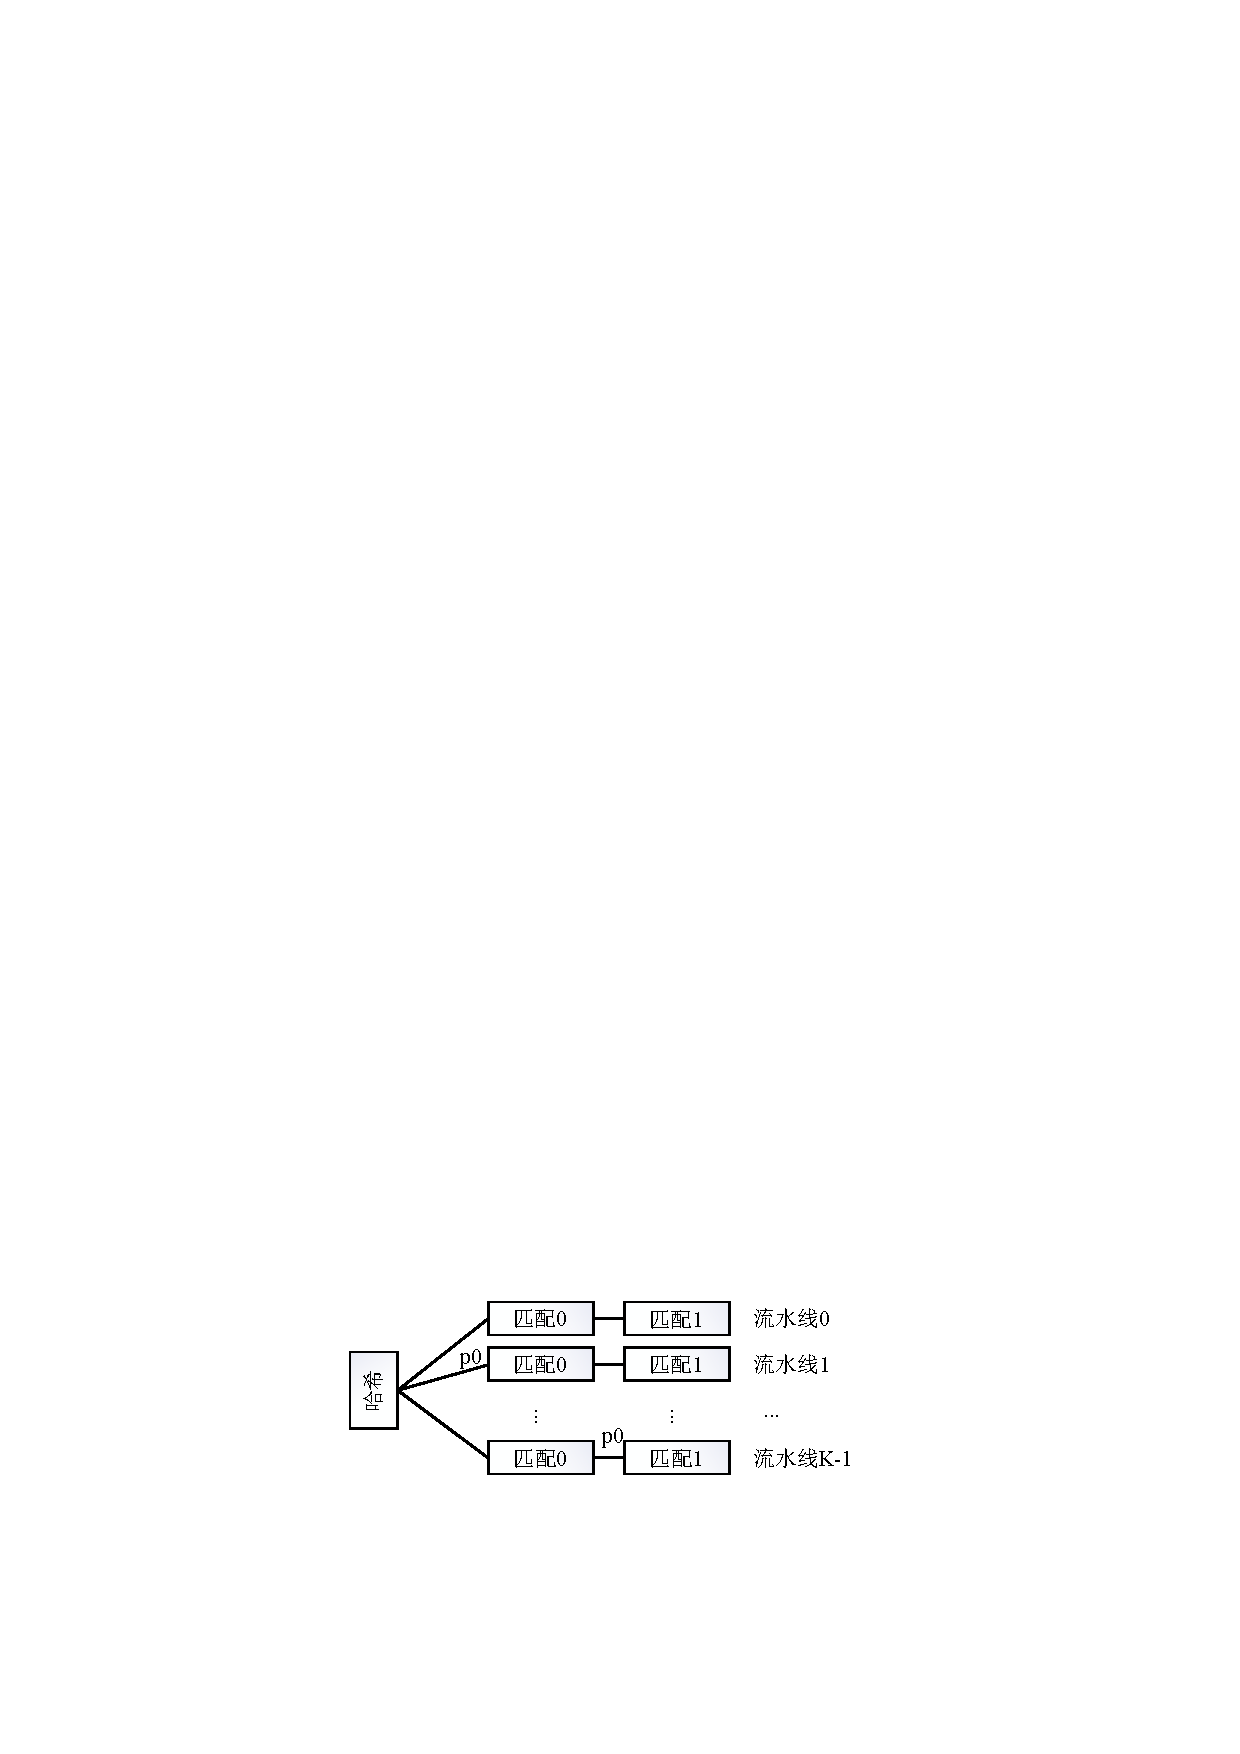
\includegraphics[scale=1]{pllb0.pdf}
	\caption{流表分割引发的数据包处理信息丢失问题} \label{fig:pllb0}
\end{figure}

为解决此问题,本文提出一种新的“并行查找块结构”,对流量均衡哈希函数以及多级流表之间数据传递进行的重新设计。如图\ref{fig:plppl}所示,每一个查找块代替传统查找流水线内的一个流表(匹配0或匹配1)。查找块使用串行方式组成流水线。每一个查找块内都包含了流量均衡分类器。数据包首先进入分类器,分类器提取出包头域中特征位,将此数据作为哈希函数的输入值进行哈希处理得到一个8位ID数字。本文将此ID号码代表前文提到的流分类组份$ j $的值。接下来的RAM表中保存了对每一个ID编号应该由哪一个子表查找的信息。数据包得到子表编号之后,通过一个交换网络转发到对应的子表流水线中,并完成相应域的查找-执行动作。分类器中子表的映射关系直接关系到后续子流水线的查找任务负载程度,以及子表中存储的流表项数目大小。

\begin{figure}[!ht]
	\centering 
	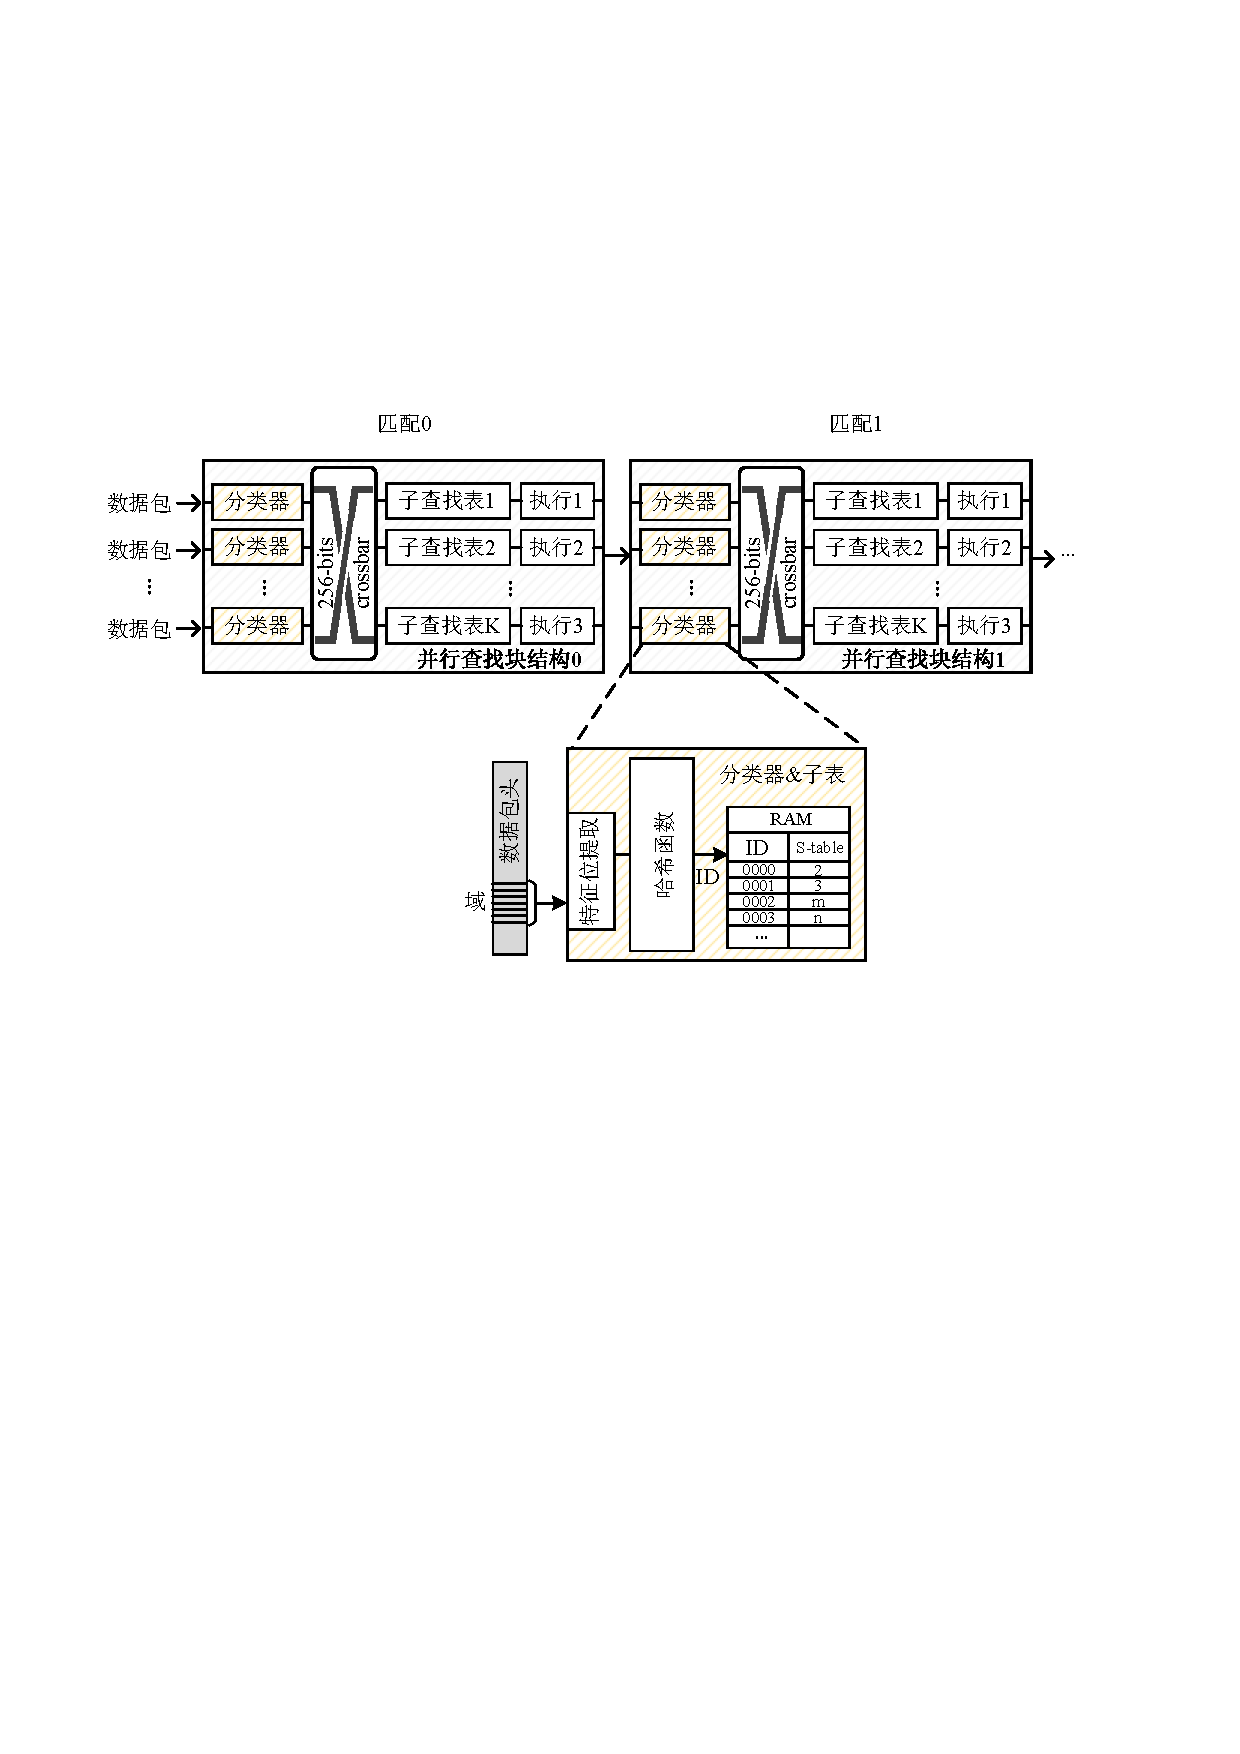
\includegraphics[scale=0.95]{plppl.pdf}
	\caption{PL端带有流量均衡的并行查找块结构} \label{fig:plppl}
\end{figure}

本结构解决了本小结前述的挑战,增加了并行处理性能,同时能够减少复制流表所耗费的资源空间。但也引入了一系列其他结构,如分类器,交叉开关以及多路执行机构。接下来本文分析这些子模块的设计复杂度以及逻辑资源开销。


\begin{itemize}
	\item 分类器。分类器由特征提取器,哈希函数以及一个查找子表组成。特征提取器和哈希函数结构简单,特征提取器在电路中使用一个固定位选路器即可实现。哈希函数使用一些异或门电路以及少量加法逻辑可实现,资源占用可以忽略不计。查找子表是本模块消耗资源最大的,但对于一般流量,只需要将其分为256或1024($j$)类即可。其最多占用存储容量1KB,现代通用型FPGA的存储资源多大上百兆,因此也可以忽略不计。
	\item 执行器。执行器内无须占用大面积存储资源,一些处理和控制功能属简单逻辑,因此执行器所消耗资源也微乎其微。
	\item 交叉开关。交叉开关可为$ K $个输入通道与$ K $个输出通道同时互相连接。是一种高性能的信息交换机制。交叉开关为每个输入与输出接口都放置了一个连接开关机构,因此一个$ K $口输入输出交叉开关需要$K^2$个逻辑资源复杂度。本文在设计并行查找块时,其并行数量$ K $在4--8个之间,因此交叉开关的资源耗费量也在可控范围内。
\end{itemize}

本文将在本章的\ref{spe4}小结中给出以上几类模块的资源消耗,从数据可以看出,本文引入的模块与流表容量相比是可以忽略不计,因此设计是有效的。
本文对一般结构的数据包处理流水线做了两方面的优化。在横向上,每条子流水线包含了多级查找表设计;纵向上,每条流水线之间的同一级流表中流表项以分散的形式存储在子流表内。本文并不改变传统的查找表与执行机构的设计,只改变了其组织和使用方式,因此查找表依然可以使用目前工具链由高层次语言编译。因此在PL的编译中,本文的前端编译器只需要将流表定义转译为拆分后的结构。其他的辅助模块结构是固定的无需再修改,这也为本文的前端编译器设计工作减轻了负担。通过以上两种优化方法,本文可同时享受到并行包处理流水线带来的高吞吐量,也无需大量复制流表项,且能保证流表资源不成倍增长。


%
%有状态转发放到实验中去讲

\BiSection{软件设计}{aa}

对本文提出的自适应交换系统的编程涉及到两个部分,一部分是分类器子表的配置,另一部分是流表项的配置。由前文分析可知,分类器子表的配置影响到后续子流水线中流量分配,以及子表中流表项数目的占用。而且如果更改子表配置,则后续对应的子流水线流表项也许同步进行删除和添加。分类器子表的配置是根据不同流组份流量大小来确定的。根据真实流量的分析\citeup{zheng2006tcam},平均情况下一个流组份的流量大小基本保持不变。因此在得到最佳配置之前,可以先通过测量的方式来对分类配置进行实时调整。接下来本文分析分类表以及流表配置过程。

在哈希函数将数据包分类到j个组份之后,每个组份的平均流量大小是随机的,且不均匀。分配过程的主要任务是将各个组份分配到K条子流水线之后使子流水线中的流量尽量保持均衡。此外,每个组份所包含的流个数也不尽相同,但每一条子流表的深度是相同的(假设为原来匹配流表深度的$ 1/K $),分配过程还应注意到不同类别的流表拆分会导致流表多份复制,且应该使得每个子流表中所分配到的流表项数目均衡,并最大限度地减少流表资源的额外消耗。

未解决上述的多约束问题,本文首先将问题数学抽象:对于图\ref{fig:plppl}中所示的一个并行查找结构。假设$N_0$是这一级匹配拆分前所对应的原始流表项数目;$C_0$是原始流表容量深度;$R_d$是流表的资源消耗率;$N$是并行流表中流表中已消耗的资源总量;$K$是流水线并行度;$C_k(k\in [1,K])$是每个子表的设计容量;分组$ ID $号码由HASH()函数求得,且$ j=HASH(P~bits) $,输入数据是一个$ P $位宽度的数值,$ j $表示了$ ID $值的空间范围。

因此可以得到对于流表资源的总约束条件:

\begin{equation} \label{pl2}
N \leq \sum_{k=1}^{K}C_k \leq C_0 \times R_d
\end{equation}

假设 $D\_flow[i]$是网络中数据包流$ i $的流量大小,则有:

\begin{equation} \label{pl3}
\sum_{i=1}^{N}D\_flow[i]=1,i \in [i,N]
\end{equation}

$D\_id[j]$是属于同一个ID分组内的总流量大小:

\begin{equation} \label{pl3}
D\_id[j]=\sum_{flow[i]\in j}^{}D\_flow[i]
\end{equation}

$T$被定义为一个并行查找块内分布式子表的总流表空间占用超出原始用量的比例。由于对FPGA内总资源的把控需求,可为流表多倾斜分配的资源有一个上限,可用$T$来表达。令$S$是组份j所组成的集合,$S={1,2,\cdots,2^P}$。$Q_k$定义为每个哈希后ID组份的最终分配情况,$Q_k \in S$,$\cup Q_k=S$, $|Q_k|$表示一个子流表中组份的总个数。令$D[k]$为第k个子流水线所承载的总数据包吞吐,则有:

\begin{equation} \label{pl3}
D[k]=\sum_{j\in Q_k}D\_id[j]
\end{equation}

如前文(流表拆分)中分析,一个带有掩码的流表项可被拆分到不同的组份$ j $中,但其中不同的组份还有可能被重新分配到同一个子流表内。因此可以将已经拆分开的掩码表项重新合成一条。定义总共被合并掉的表项个数为$V_k$。本文称待解决优化问题为“基于流量均衡的流表组合问题”。


\noindent 将基于流量均衡的流表组合问题形式化如下,若服从:



$Q_{k}\subseteq S, k\in \left[ 1,k\right],\cup Q_{k}=S;\sum ^{k}_{i=1}C_{k}\left[ i\right] \leq C_{0}\cdot R_{d} $

$\left| \left| \dfrac {Q_{i}}{C_{ki}}\right| -\left| \dfrac {Q_{j}}{C_{kj}}\right| \right|\cdot 100\%\leq T\left( i, j, ki, kj\in \left[ 1,k\right] \right) $

$ BOOL\left(i,j\right)=
\begin{cases}
1& \text{ $j \in Q_i$ }\\
0& \text{ $j \notin Q_i$}
\end{cases}$

$G\left[ j\right] =\sum ^{k}_{i=1}BOOL\left( i,j\right) =1\left( j\in S\right)  $

$\sum _{j\in S}G\left[ i\right] =2^{P}\left( j\in S\right)  $

$D\left[ k\right] =\sum _{j\in Q_{k}}D_{-}id\left[ i\right] \left( k=1,\ldots ,K\right)  $

$ F_{1}\left[ k\right] =MAX\left( D\left[ k\right] \right) -MlN\left( D\left[ k\right] \right) \leq q_1$

$ F_{2}\left[ k\right] =C_{0}-\sum ^{K}_{k=1}V_{k}\leq q_{2}$


\noindent 求一种帕累托方程优化最小值:

\begin{equation} \label{pl3}
 F\left[ k\right] =\left( F_{1}\left[ k\right] ,F_{2}\left[ k\right] \right) \left( k\in \left[ 1,K\right] \right) 
\end{equation}


本文将证明上述问题为NP难解问题,而后给出一种基于模拟退火的启发式算法。首先引入一个经典的NP完全问题“平均分割问题”,随后本文通过给出此问题的退化过程,证明“基于流量均衡的流表组合问题”是一个NP难问题。

\begin{theorem}%[Riesz 表示定理]
	$K$为系统并行流水线数目,当$k\in [1,K]$,对于待求问题\ref{label}
	$ c $为公式\ref{mydiscof7}中的统计值,其中$ f(c) $为真实统计量的估计值,则$ f(c) $是一种无偏估计。即,对任意$ i\in N^{\ast} $,有:
	\begin{equation} \label{mydiscof8}
	E[f(c_i)]=\sum ^{m}_{i=1}l_{i}
	\end{equation}	
\end{theorem}

\begin{proof}
	首先,考虑函数$ f(c) $的第一阶段。由于线性计数,计数值等于累加值,存在特殊情况$n$($ n\leq m $),使得:
	
	\begin{equation} \label{mydiscofa}
	c_i=\sum ^{k}_{i=1}l_{i} \quad\quad k \leq n; k,n,m \in N^{\ast}
	\end{equation}
	
	又根据定义(公式\ref{mydiscof7}),可得:
	
	\begin{align}\label{mydiscofb}
	f(c_i) &= c_i \nonumber \\
	&=\sum ^{k}_{i=1}l_{i} \quad\quad k \leq n
	\end{align}
	
	因此:
	
	\begin{align}\label{mydiscofc}
	E[f(c_i)] &= E(c_i) \nonumber \\
	&=c_i \nonumber  \\
	&=\sum ^{k}_{i=1}l_{i} \quad\quad i \leq n
	\end{align}
	
	其次,考虑第二阶段,前文工作\citeup{hu2013discount}已经证明:
	
	\begin{equation} \label{mydiscofd}
	E[\dfrac{b^c-1}{b-1}]=\sum_{i=1}^{m}l_i \quad\quad i \leq m
	\end{equation}
	
	令p为第二阶段内的某一个数据包,即$ n \leq p \leq m $,根据定义\ref{mydiscof9}可得:
	
	\begin{equation} \label{mydiscofe}
	f(c_n) = c_n = \dfrac{b^{c_n}-1}{b-1}\quad\quad p=n
	\end{equation}
	
	由\ref{mydiscofd}与\ref{mydiscofe}得到:
	
	\begin{equation} \label{mydiscoff}
	E[f(c_p)]=E[\dfrac{b^{c_p}-1}{b-1}]=\sum_{i=1}^{p}l_i\quad\quad p=n
	\end{equation}
	
	由于p=n时无偏性成立,因此当p>n时,可直接应用结论\ref{mydiscofd}得证无偏性:
	
	\begin{equation} \label{mydiscofh}
	E[f(c_p)]  = \sum_{i=1}^{p}l_i \quad\quad n<p\leq m
	\end{equation}
	
	联系\ref{mydiscofc}、\ref{mydiscoff}与\ref{mydiscofh}得到:
	
	\begin{equation} \label{mydiscofg}
	E[f(c_p)]==\sum_{i=1}^{p}l_i\quad\quad p \in [1,m]
	\end{equation}
	
	以上证明假定数据包$ 1,2,\cdots,n $恰好组成了第一阶段,且数据包$ n,n+1,p,\cdots,m $恰好组成第二阶段,并得证。另需证明一般情况,Magic\_Number无法由确定数量包长度之和组成,即:
	
	\begin{equation} \label{mydiscofi}
	\sum_{i=1}^{n}l_i < C_{magic} < \sum_{i=1}^{n+1}l_i
	\end{equation}
	
	\begin{figure}[!ht]
		\centering
		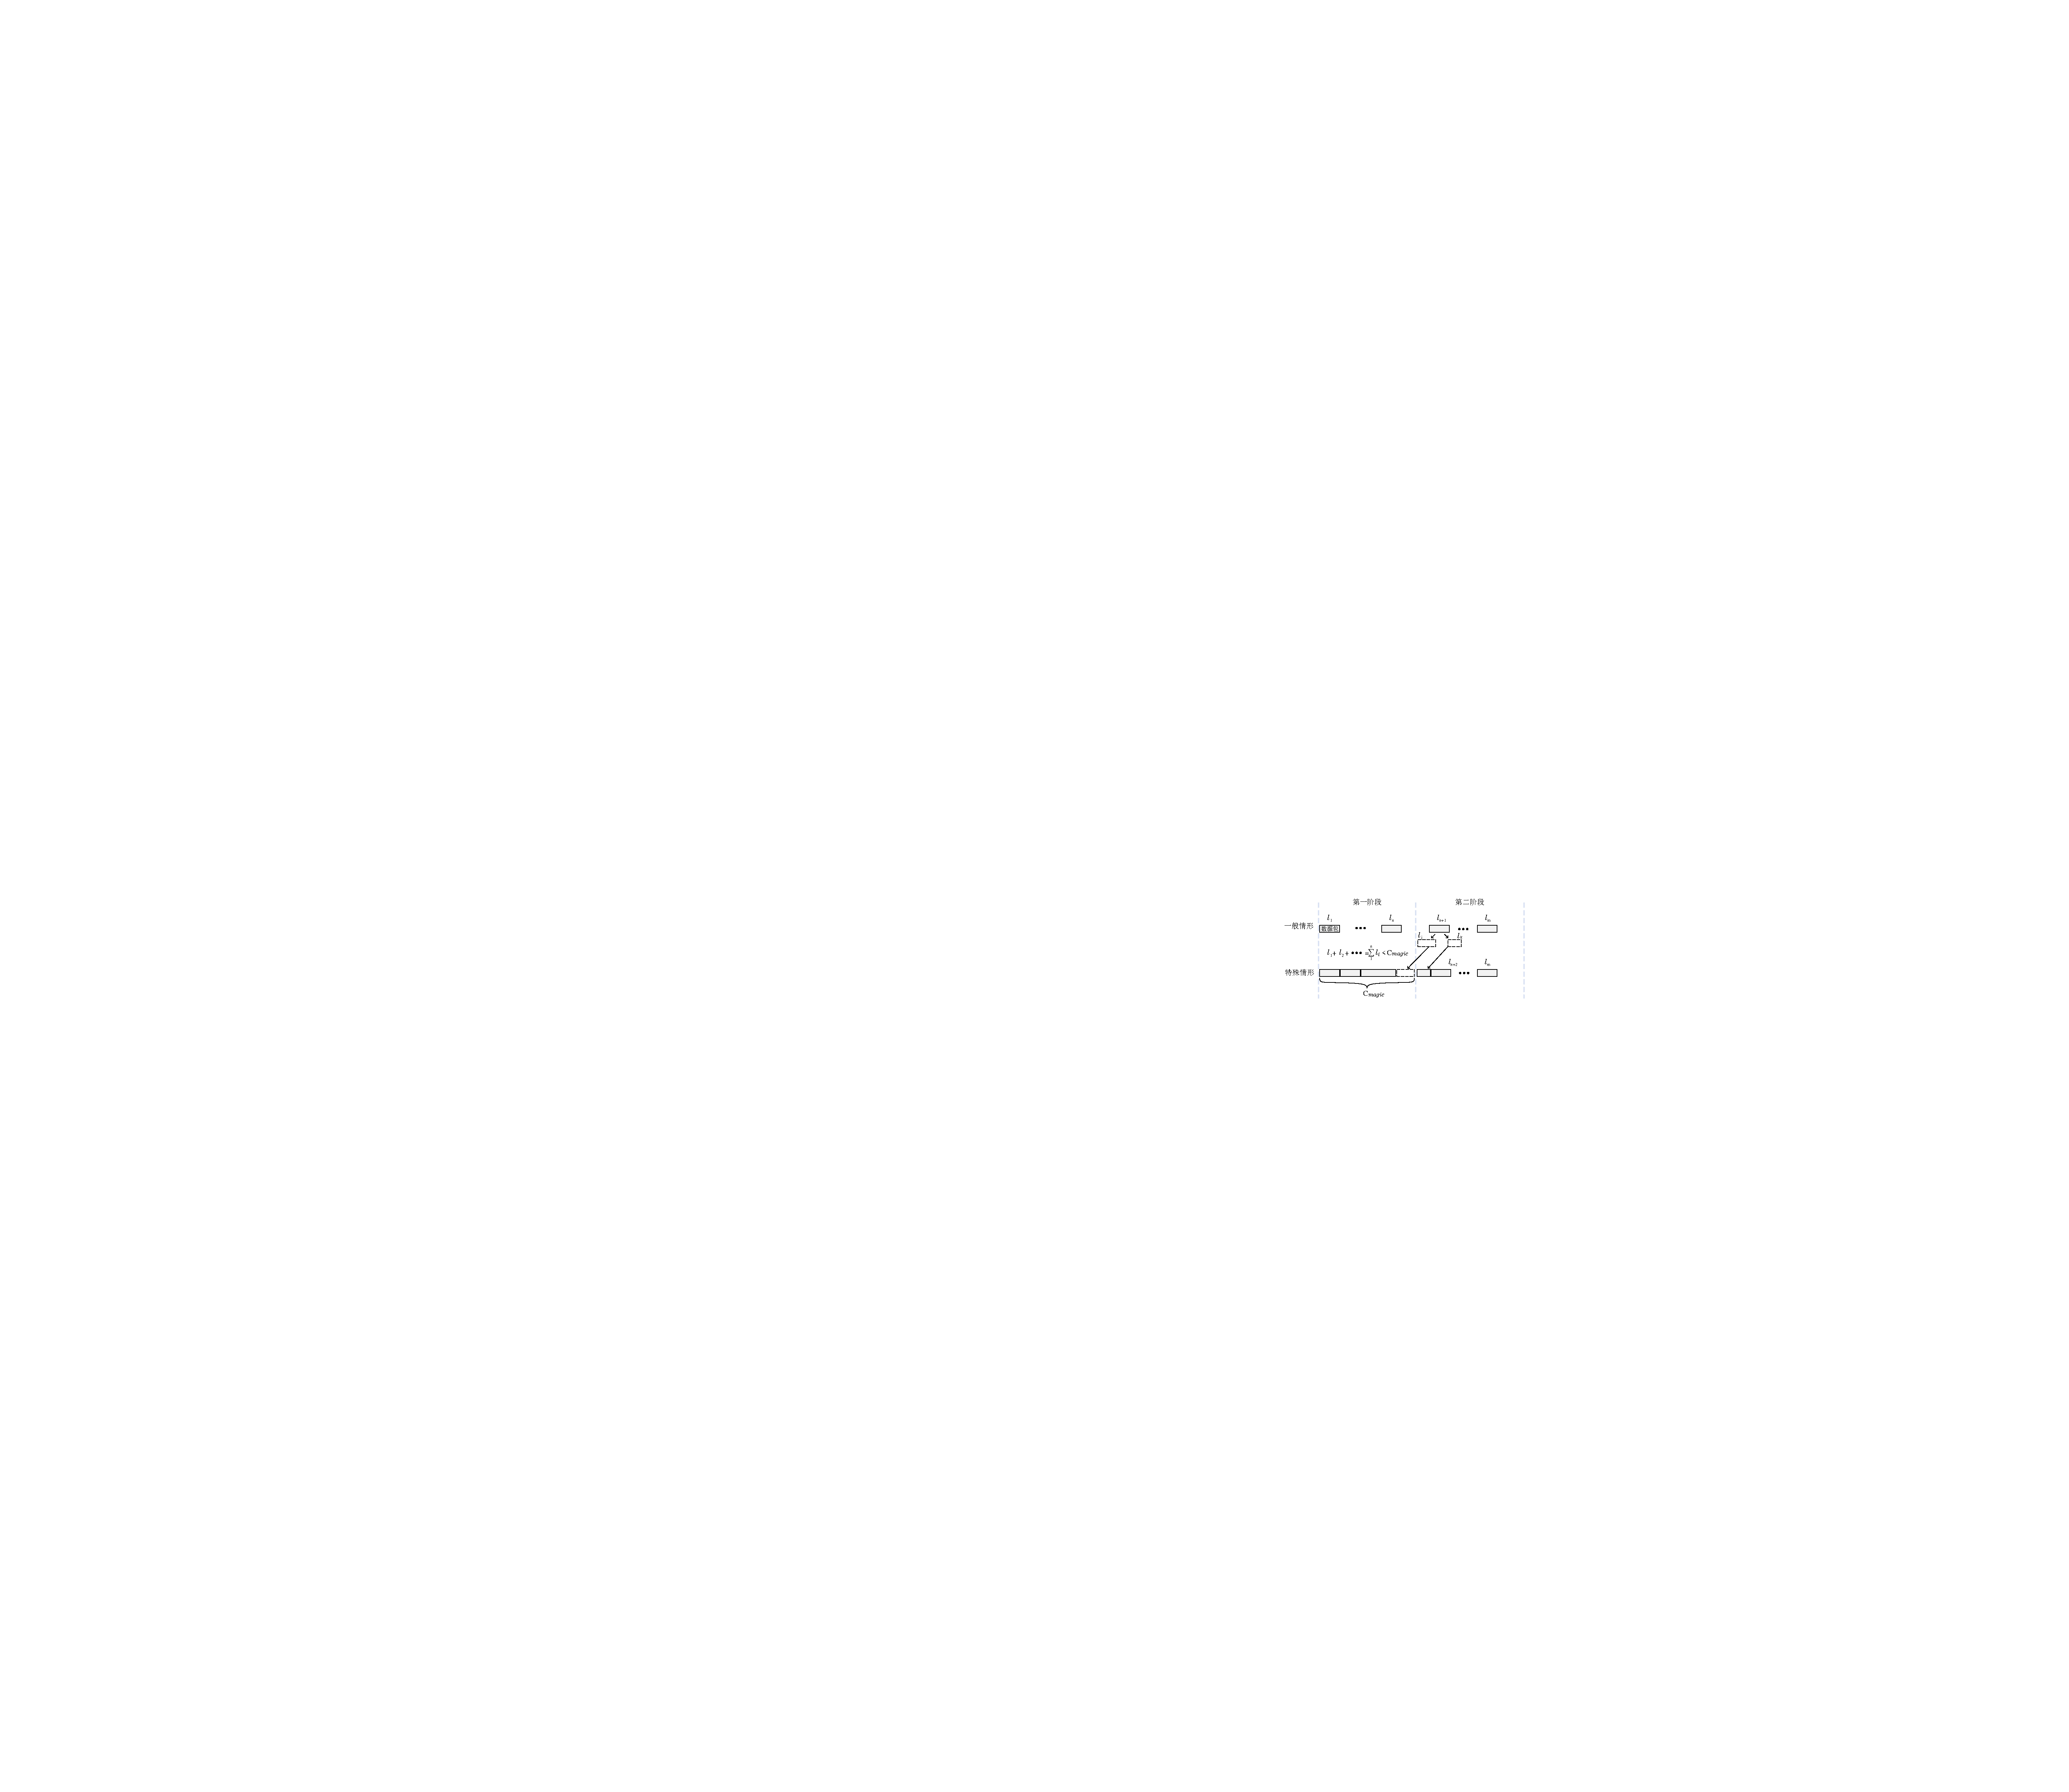
\includegraphics[scale=1]{discozhengming.pdf}
		\caption{一般情形转化为特殊情形得以证明} \label{fig:discozhengming}
	\end{figure}
	
	对此(根据算法\ref{mydiscoa4}),如图\ref{fig:discozhengming},将第$ n+1 $个数据包的包长度$ l_{n+1} $ 分为两部分:$ l_{n+1}=j+k $,得到两个序列$ n'=1,2,\cdots,n,j $,以及$ p'=k,n+1,n+2,\cdots,m $且一定有$ j $使得:
	
	\begin{equation} \label{mydiscofk}
	\left\{
	\begin{array}{rcl}
	E[f(c_{n'})]=\sum_{i=1}^{n'}l_i=\sum_{i=1}^{n}l_i+j=C_{magic}         &      & {n' \leq j} \\
	E[f(c_{p'})] =\sum_{i=1}^{p'} l_i     &      & {j\leq p' \leq m}
	\end{array} \right. 
	\end{equation}
	
	因此,归约到特殊情况的结论(\ref{mydiscofg})。证毕。
\end{proof}













NP难题


\BiSection{系统性能评价}{System performance and evaluation}\label{spe4}





\BiSection{本章小结}{aa}





